\chapter{Experimental Results}
\textit{Before showing the results, it should be noted that all experiments are done by using the setup that was used for other purposes (deep sea mining) and so scaling was not good possible. The height of the tank is maximized to reduce bottom effects and also the SSC is reduced to reduce impulse at the bottom. This should be noted before comparing with prototype scales.} \newline \newline

\noindent In this chapter, the results from the experiment are analyzed. The analysis is divided into two parts, where one part consists of the concentration measurements to visualize the profile on the bottom plate, another to determine an entrainment coefficient by using the jet angle and to see differences in travel time with different nozzle shapes.


%Direct uit tests
%concentratie profielen (matlab file)
%bovenaanzicht

\newpage
\section{Concentration measurements}
As said in chapter \ref{ch:test_setup}, the concentration of the plume is measured at the bottom of the reservoir with drain points in the plate which connects to taps outside the reservoir, where the concentration is measured with the AL450T-IR Turbidity Meter. For each nozzle shape, five concentration measurements are done. An overview of all measurements and an average are visible in appendix \ref{app:Concentration}.

\subsection{Radial dispersion plume}
As shown in figure \ref{fig:Round_Lee}, an expectation of the plume width was made based on the model of \cite{Lee+}. Using the topview camera images, the measurement points can be distinguished from the plume and plate. In figure \ref{fig:topview} an topview image is shown between all three nozzle shapes.

\begin{figure}[ht!]
\centering
\begin{subfigure}{.3\textwidth}
  \centering
  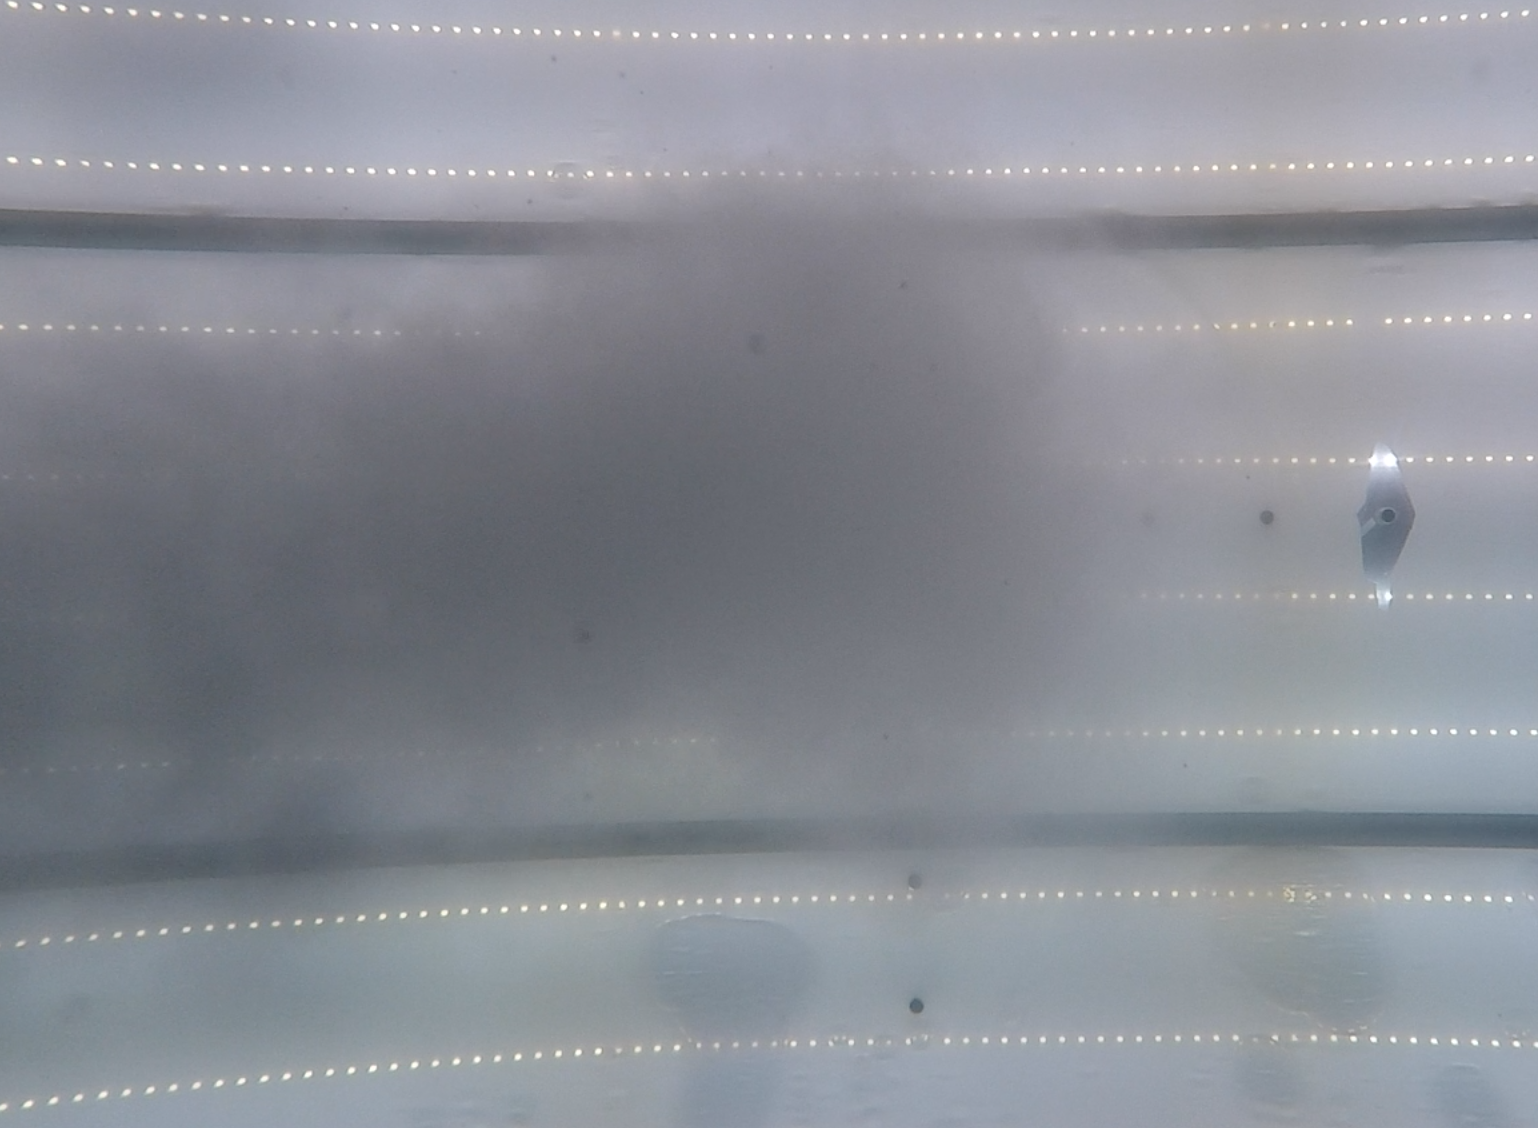
\includegraphics[width=.9\linewidth]{Images/Snapshot_Topview_Rond.png}
  \subcaption{Round}
\end{subfigure}
\begin{subfigure}{.26\textwidth}
  \centering
  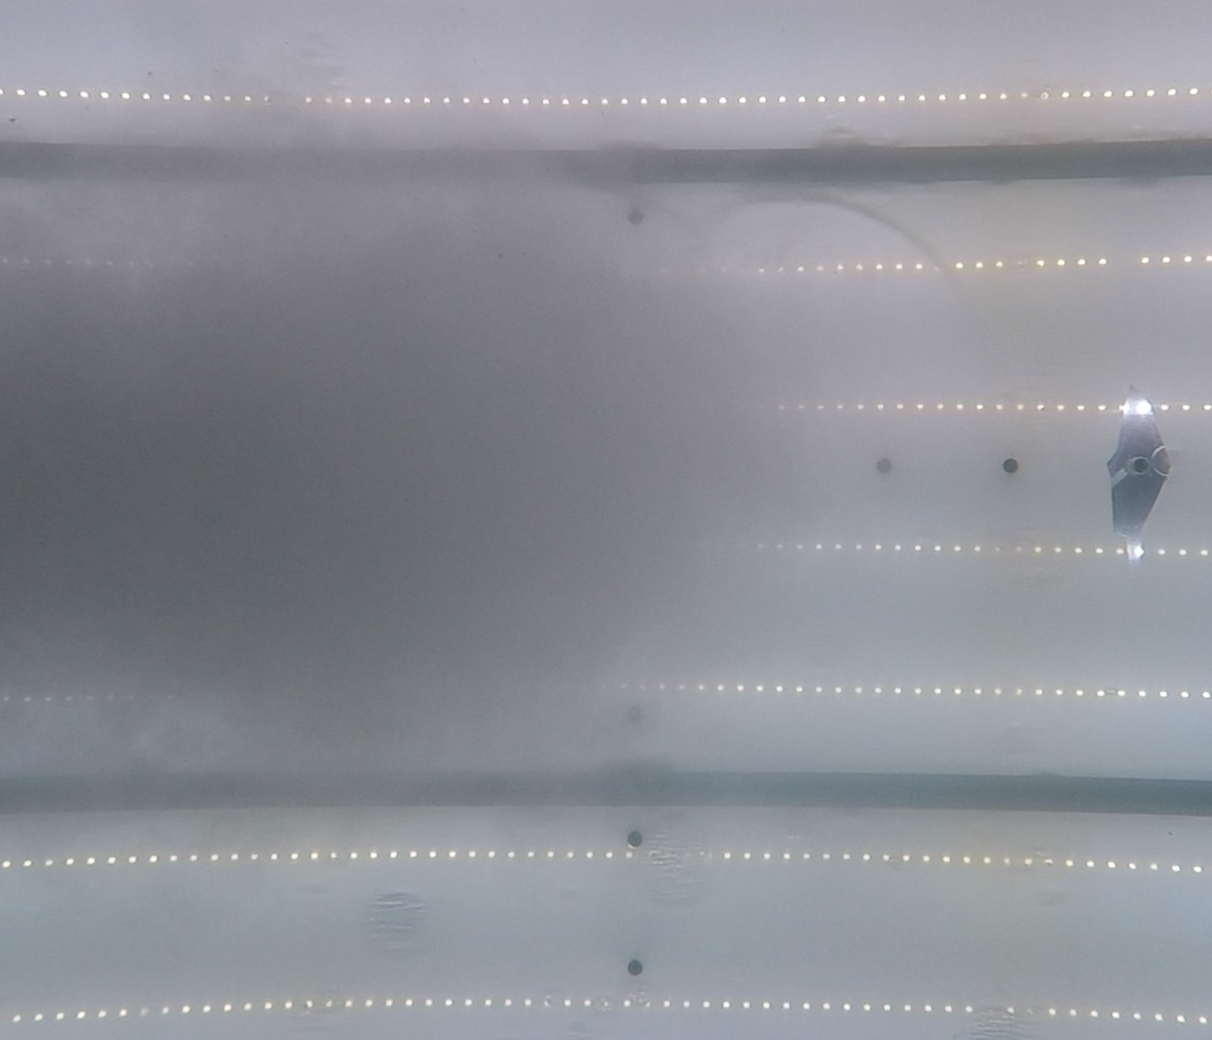
\includegraphics[width=.9\linewidth]{Images/Snapshot_Rechthoek_20x39.png}
  \subcaption{Rectangular 20x3.9}
\end{subfigure}
\begin{subfigure}{.24\textwidth}
  \centering
  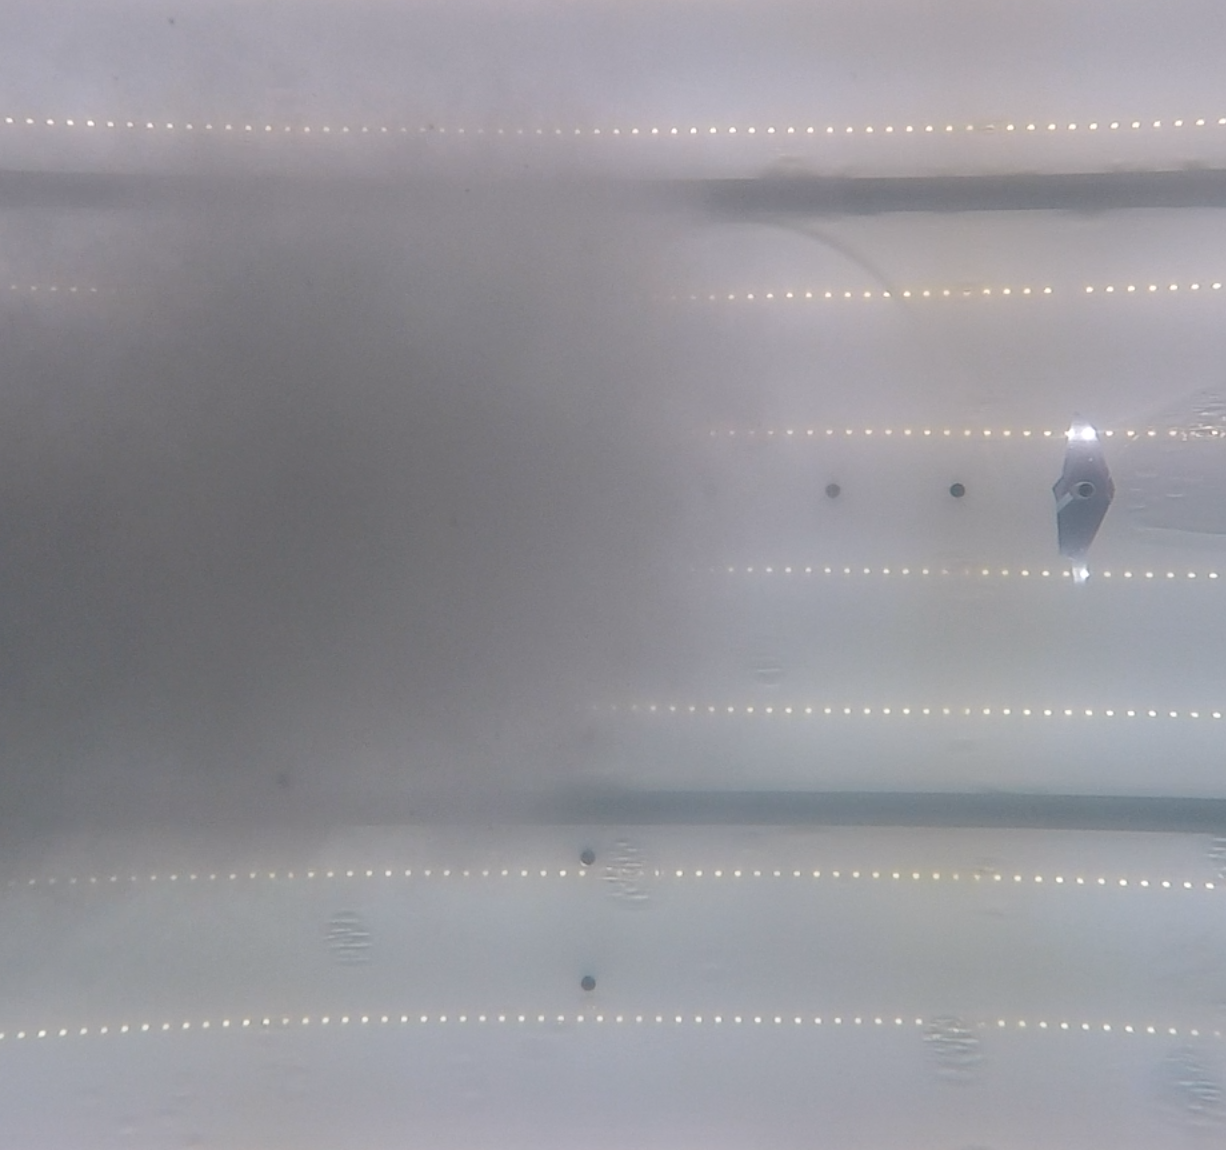
\includegraphics[width=.9\linewidth]{Images/Snapshot_Rechthoek_30x26.png}
  \subcaption{Rectangular 30x2.6}
\end{subfigure}
\caption{Topview image for all nozzle shapes}
\label{fig:topview}
\end{figure}

\noindent As shown in figure \ref{fig:topview}, it is visible that in all cases, the radius of the plume has a maximum of roughly 200mm where all measurement points with a larger radius are clearly visible. Is it also visible that a rectangular nozzle shape decreases the radius of the plume to roughly less than 100mm (more measurement points are clearly visible). With this noted, the measurement points can be divided into two parts, where some points have a plume from above and a plume current due to the table, which spreads radially on the table. The measurement points which are not visible due to the plume are assumed to have a flow from above and a current sideways due to the table. The measurement points which are clearly visible from the topview image are assumed to have only a sideways current due to table. \newline
\noindent Due to the current, some concentrations measured with the turbidity meter are not representative to give a conclusive result. Looking at figure \ref{fig:topview}, all measurement points with a radius > 200mm only have a concentration of a sideways current due to the bending effect of the plume, which is a effect of the tables boundary. In the case of the rectangular nozzles, the radial dispersion is even less. Therefore it is harder to give representative conclusions of measuring points with a radius of > 100mm which will increase change of fluctuation in the results of the concentration measurements. \newline
\noindent Connecting this with the model from \cite{Lee+} (figure \ref{fig:Round_Lee}) which does not have the effect of a hard boundary and the concentration measurements, where some points have a vertical plume and horizontal current effect, the measurement concentrations should show a higher concentration due to the horizontal current added. Looking at a radius of 200mm between the models value (30 mg/l) and the averaged measured concentration at this point in case of a round overflow shape, which has a vertical plume flow and horizontal current, which is 40.64 mg/l (see appendix \ref{app:Concentration}), an added value is shown which can be translated to the horizontal current. Noting that a value > 30 mg/l should be found at this radius gives that the concentration measurements satisfies this. \newline


\noindent Due to the radial dispersion measured and the connection with the measurement points, it is chosen to focus the concentration measurement on the points with a radius of 100mm, which are the points closest to the middle point.

\subsection{Concentration profile bottom plate}
%matlab file zijaanzicht
%matlab file bovenaanzicht
%verschil in gemeten concentratie

Focusing on the measurement points with a radius of 100mm, which are points 4,5,9 and 11, the measured concentration in case of all nozzle shapes are found in table \ref{tab:round_concentration} (Round), table \ref{tab:rec20_concentration} (Rectangular 20x3.9) and table \ref{tab:rec30_concentration}. The numbers shown are the averaged results of each test, which are again averaged to get one value of all tests. The total averaged NTU is then converted to mg/l.


\begin{table}[ht!]
\centering
\begin{tabular}{|c|c|c|c|c|c|c|c|}
\hline
\multicolumn{8}{|c|}{\textbf{Round}} \\ \hline
\textbf{Measurement point} & \textbf{Test 1} & \textbf{Test 2} & \textbf{Test 3} & \textbf{Test 4} & \textbf{Test 5} & \textbf{Average NTU} & \textbf{Average mg/l} \\ \hline
4 & 13.92 & 11.88 & 9.25 & 10.54 & 10.57 & 11.23 & 46.32 \\ \hline
5 & 13.33 & 12.81 & 9.79 & 11.14 & 10.20 & 11.46 & 48.15 \\ \hline
9 & 13.50 & 13.38 & 10.45 & 10.87 & 10.44 & 11.73 & 50.37 \\ \hline
11 & 12.88 & 12.02 & 10.00 & 10.55 & 10.46 & 11.18 & 45.89 \\ \hline
\end{tabular}
\caption{Average results of all 5 tests done with round nozzle shape}
\label{tab:round_concentration}
\end{table}

\begin{table}[ht!]
\centering
\begin{tabular}{|c|c|c|c|c|c|c|}
\hline
\multicolumn{7}{|c|}{\textbf{Rectangular 20x3.9}} \\ \hline
\textbf{Measurement point} & \textbf{Test 1} & \textbf{Test 2} & \textbf{Test 3} & \textbf{Test 4} & \textbf{Average NTU} & \textbf{Average mg/l} \\ \hline
4 & 12.54 & 12.07 & 13.13 & 13.20 & 12.74 & 58.61 \\ \hline
5 & 12.57 & 12.04 & 11.63 & 13.44 & 12.42 & 56.04 \\ \hline
9 & 13.87 & 12.66 & 11.96 & 13.78 & 13.06 & 61.29 \\ \hline
11 & 14.37 & 12.62 & 10.81 & 13.46 & 12.81 & 59.25 \\ \hline
\end{tabular}
\caption{Average results of all 4 tests done with rectangular 20x3.9 nozzle shape}
\label{tab:rec20_concentration}
\end{table}


\begin{table}[ht!]
\centering
\begin{tabular}{|c|c|c|c|c|c|c|c|}
\hline
\multicolumn{8}{|c|}{\textbf{Rectangular 30x2.6}} \\ \hline
\textbf{Measurement point} & \textbf{Test 1} & \textbf{Test 2} & \textbf{Test 3} & \textbf{Test 4} & \textbf{Test 5} & \textbf{Average NTU} & \multicolumn{1}{l|}{\textbf{Average mg/l}} \\ \hline
4 & 12.43 & 10.46 & 12.81 & 12.52 & 12.84 & 12.21 & 54.35 \\ \hline
5 & 13.28 & 11.88 & 11.23 & 13.69 & 12.22 & 12.46 & 56.35 \\ \hline
9 & 11.69 & 12.42 & 12.59 & 12.57 & 12.47 & 12.35 & 55.43 \\ \hline
11 & 13.69 & 13.31 & 11.28 & 14.59 & 12.28 & 13.03 & 61.00 \\ \hline
\end{tabular}
\caption{Average results of all 5 tests done with rectangular 30x2.6 nozzle shape}
\label{tab:rec30_concentration}
\end{table}
\newpage
\noindent Is is clearly shown that a rectangular nozzle shape, with the same outflow area as a round nozzle shape, shows an increase of concentration at a radius of 100mm from the middle point. Taking an average value for all four measurement points (Round = 47.68 mg/l, Rectangular 20x3.9 = 58.80 mg/l, Rectangular 30x2.6 = 56.78 mg/l) shows an increase of roughly $22\%$ in case of a rectangular nozzle shape. Looking at the aspect ratio of the rectangular nozzles, it is difficult to distinguish any difference based on only the concentration measurements. A visualisation is shown in figures \ref{fig:side_concentratie} (side) and \ref{fig:top_concentratie} (top) between the different nozzle shapes. A value of 70 mg/l is given to the middle point, which is in line with the model of \cite{Lee+}. 

\begin{figure}[ht!]
\centering
\begin{subfigure}{.33\textwidth}
  \centering
  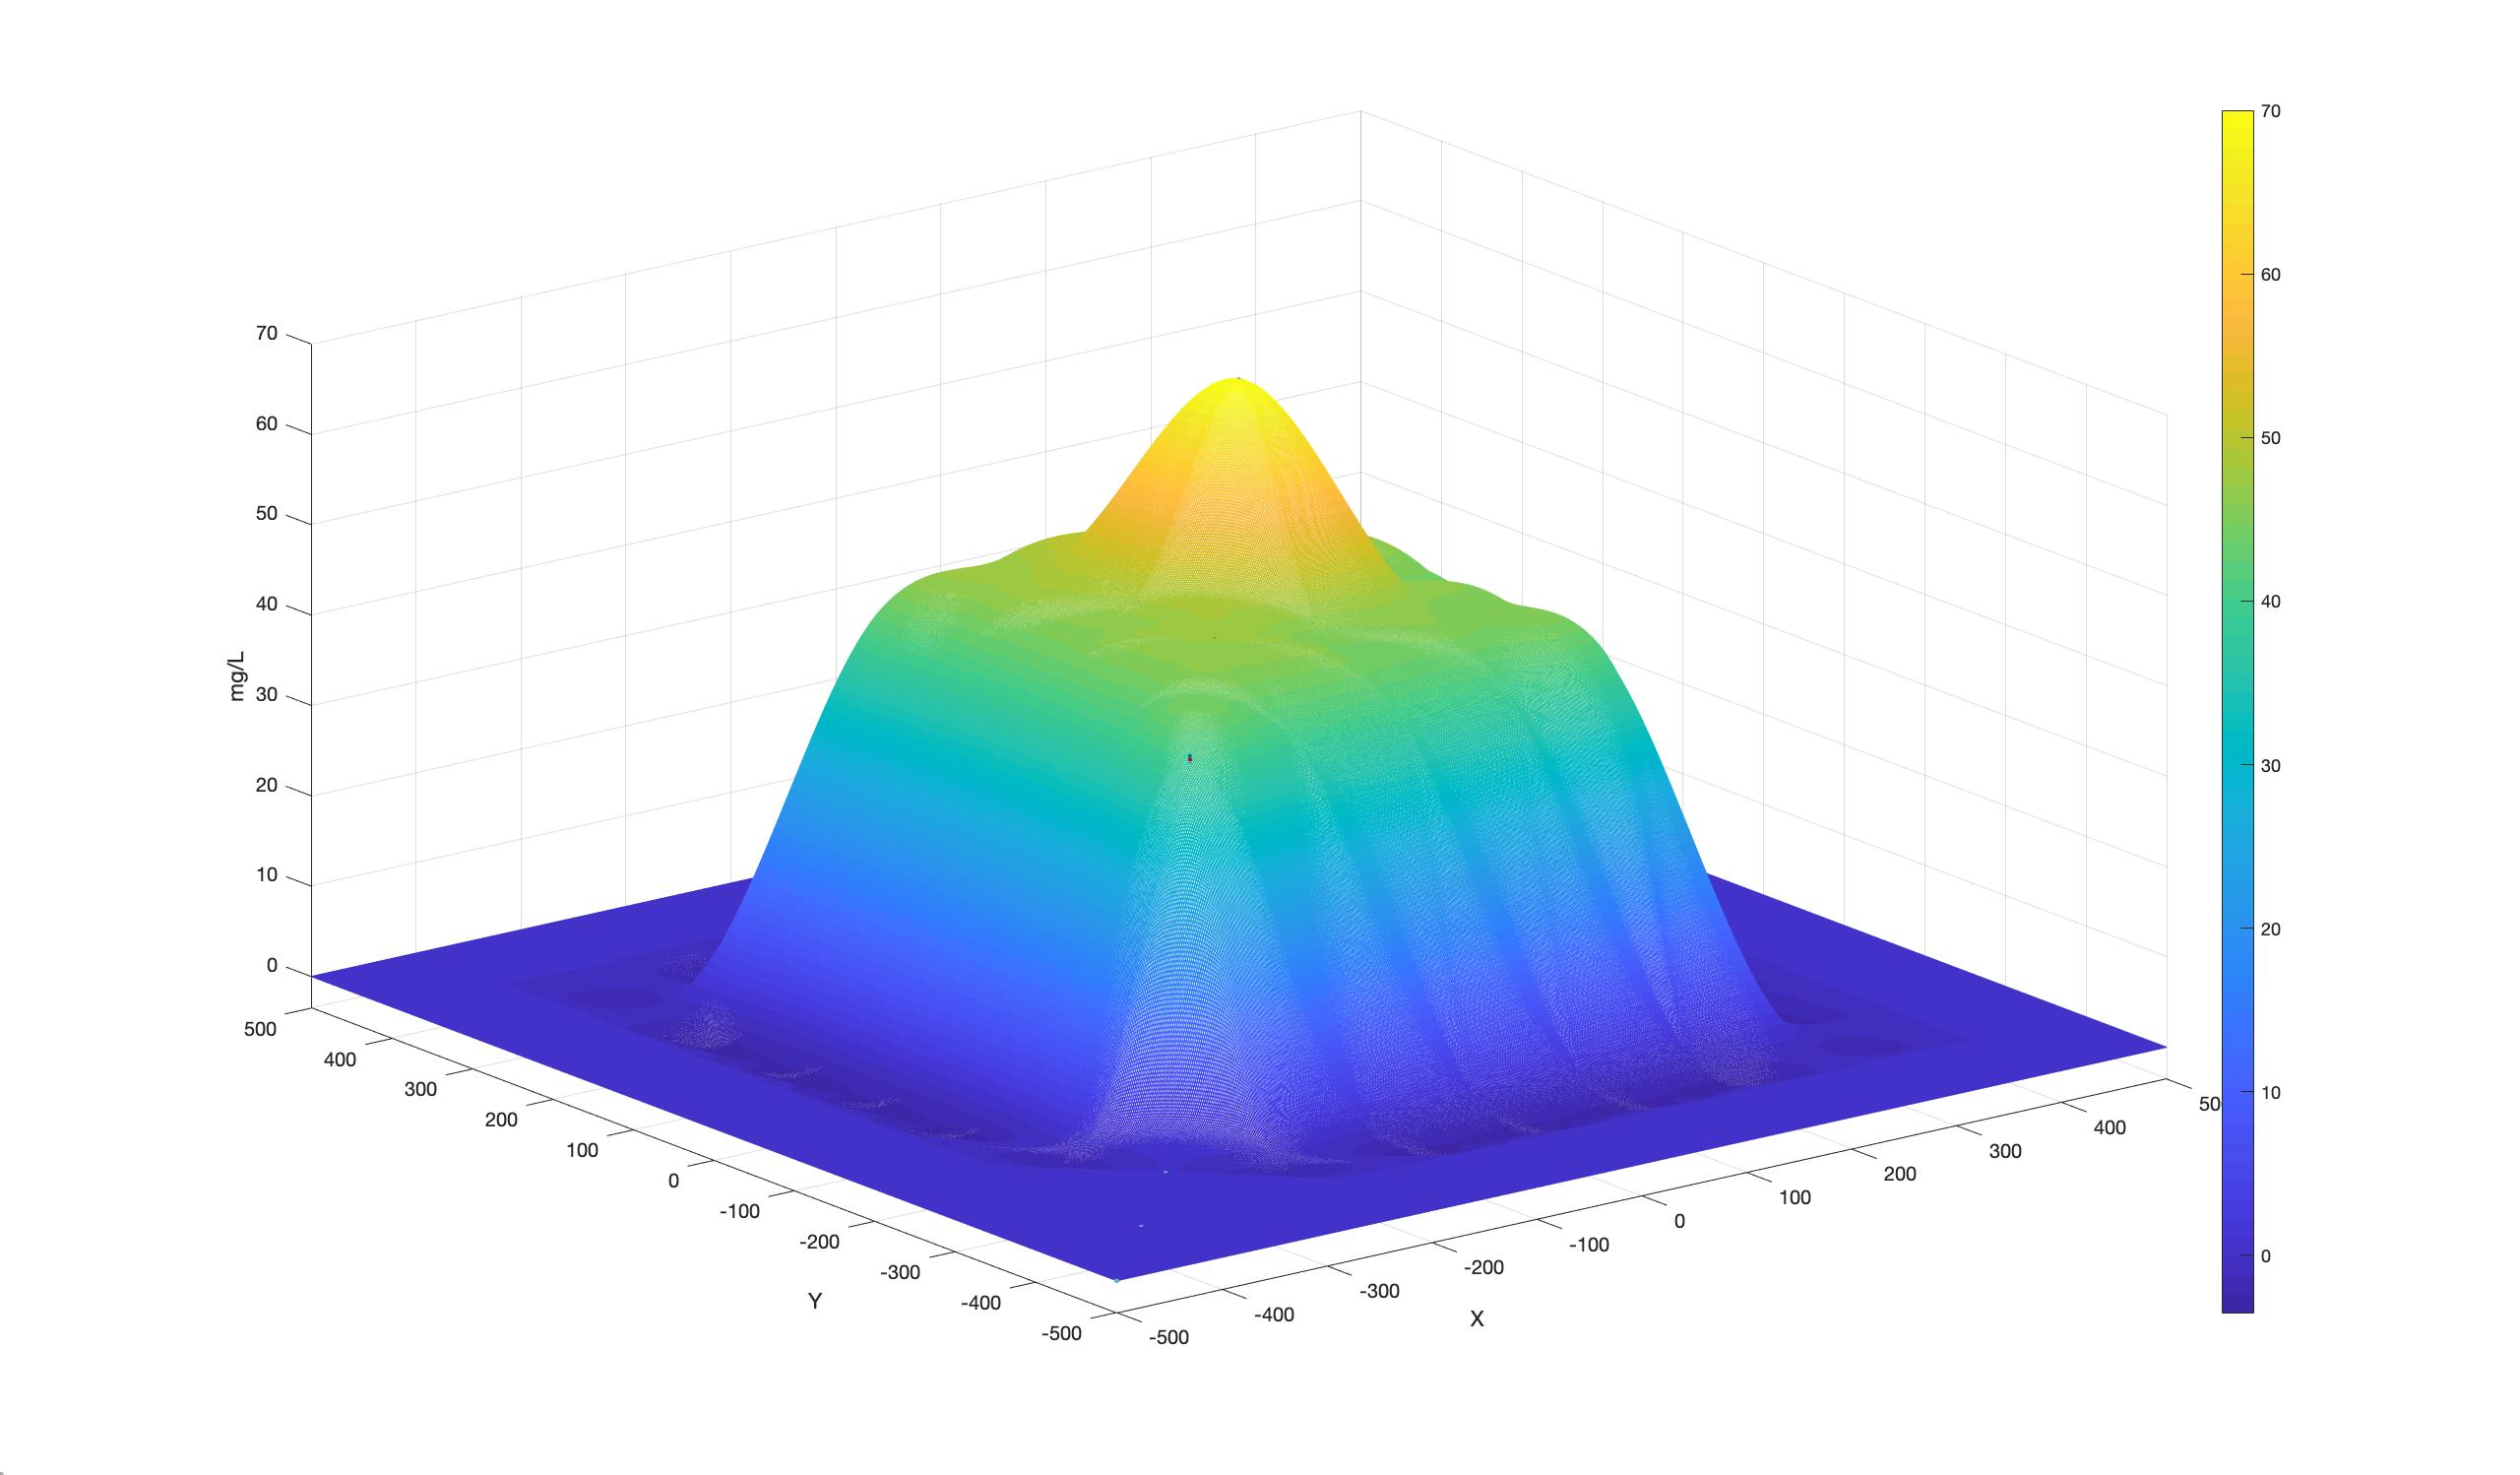
\includegraphics[width=.9\linewidth]{Images/Round_side.jpg}
  \subcaption{Round}
\end{subfigure}
\begin{subfigure}{.33\textwidth}
  \centering
  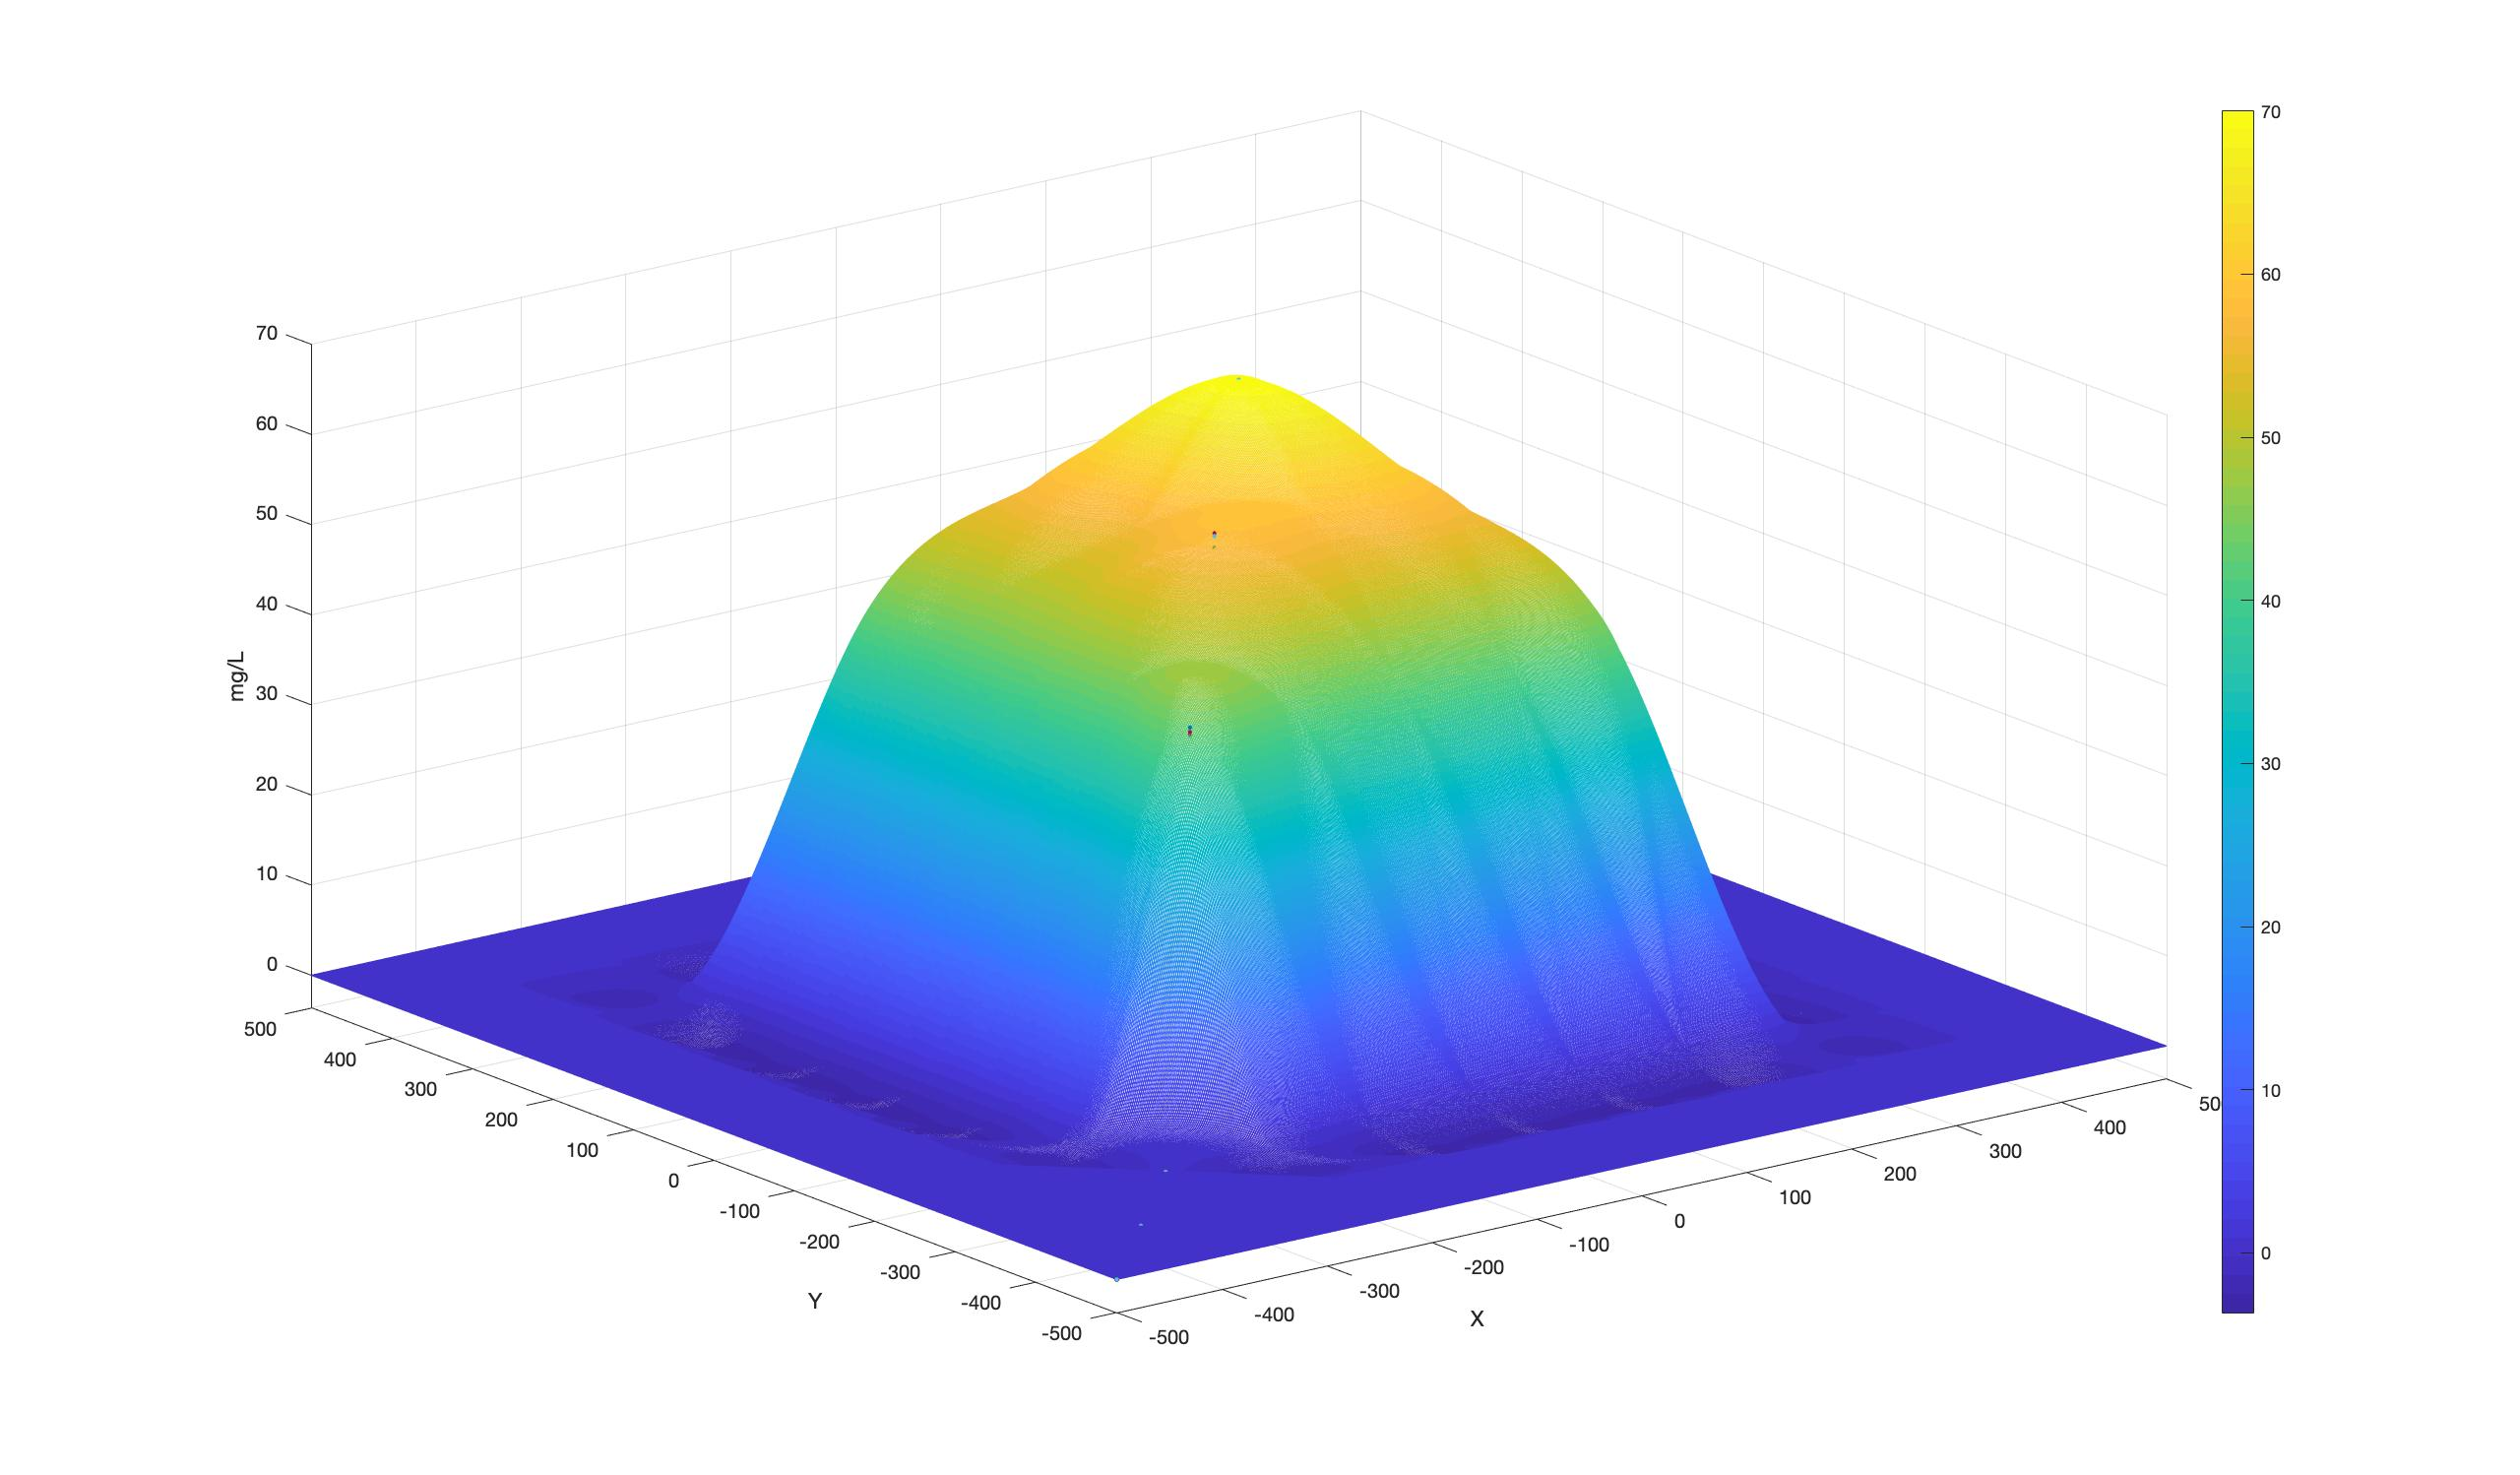
\includegraphics[width=.9\linewidth]{Images/Rec20_side.jpg}
  \subcaption{Rectangular 20x3.9}
\end{subfigure}
\begin{subfigure}{.33\textwidth}
  \centering
  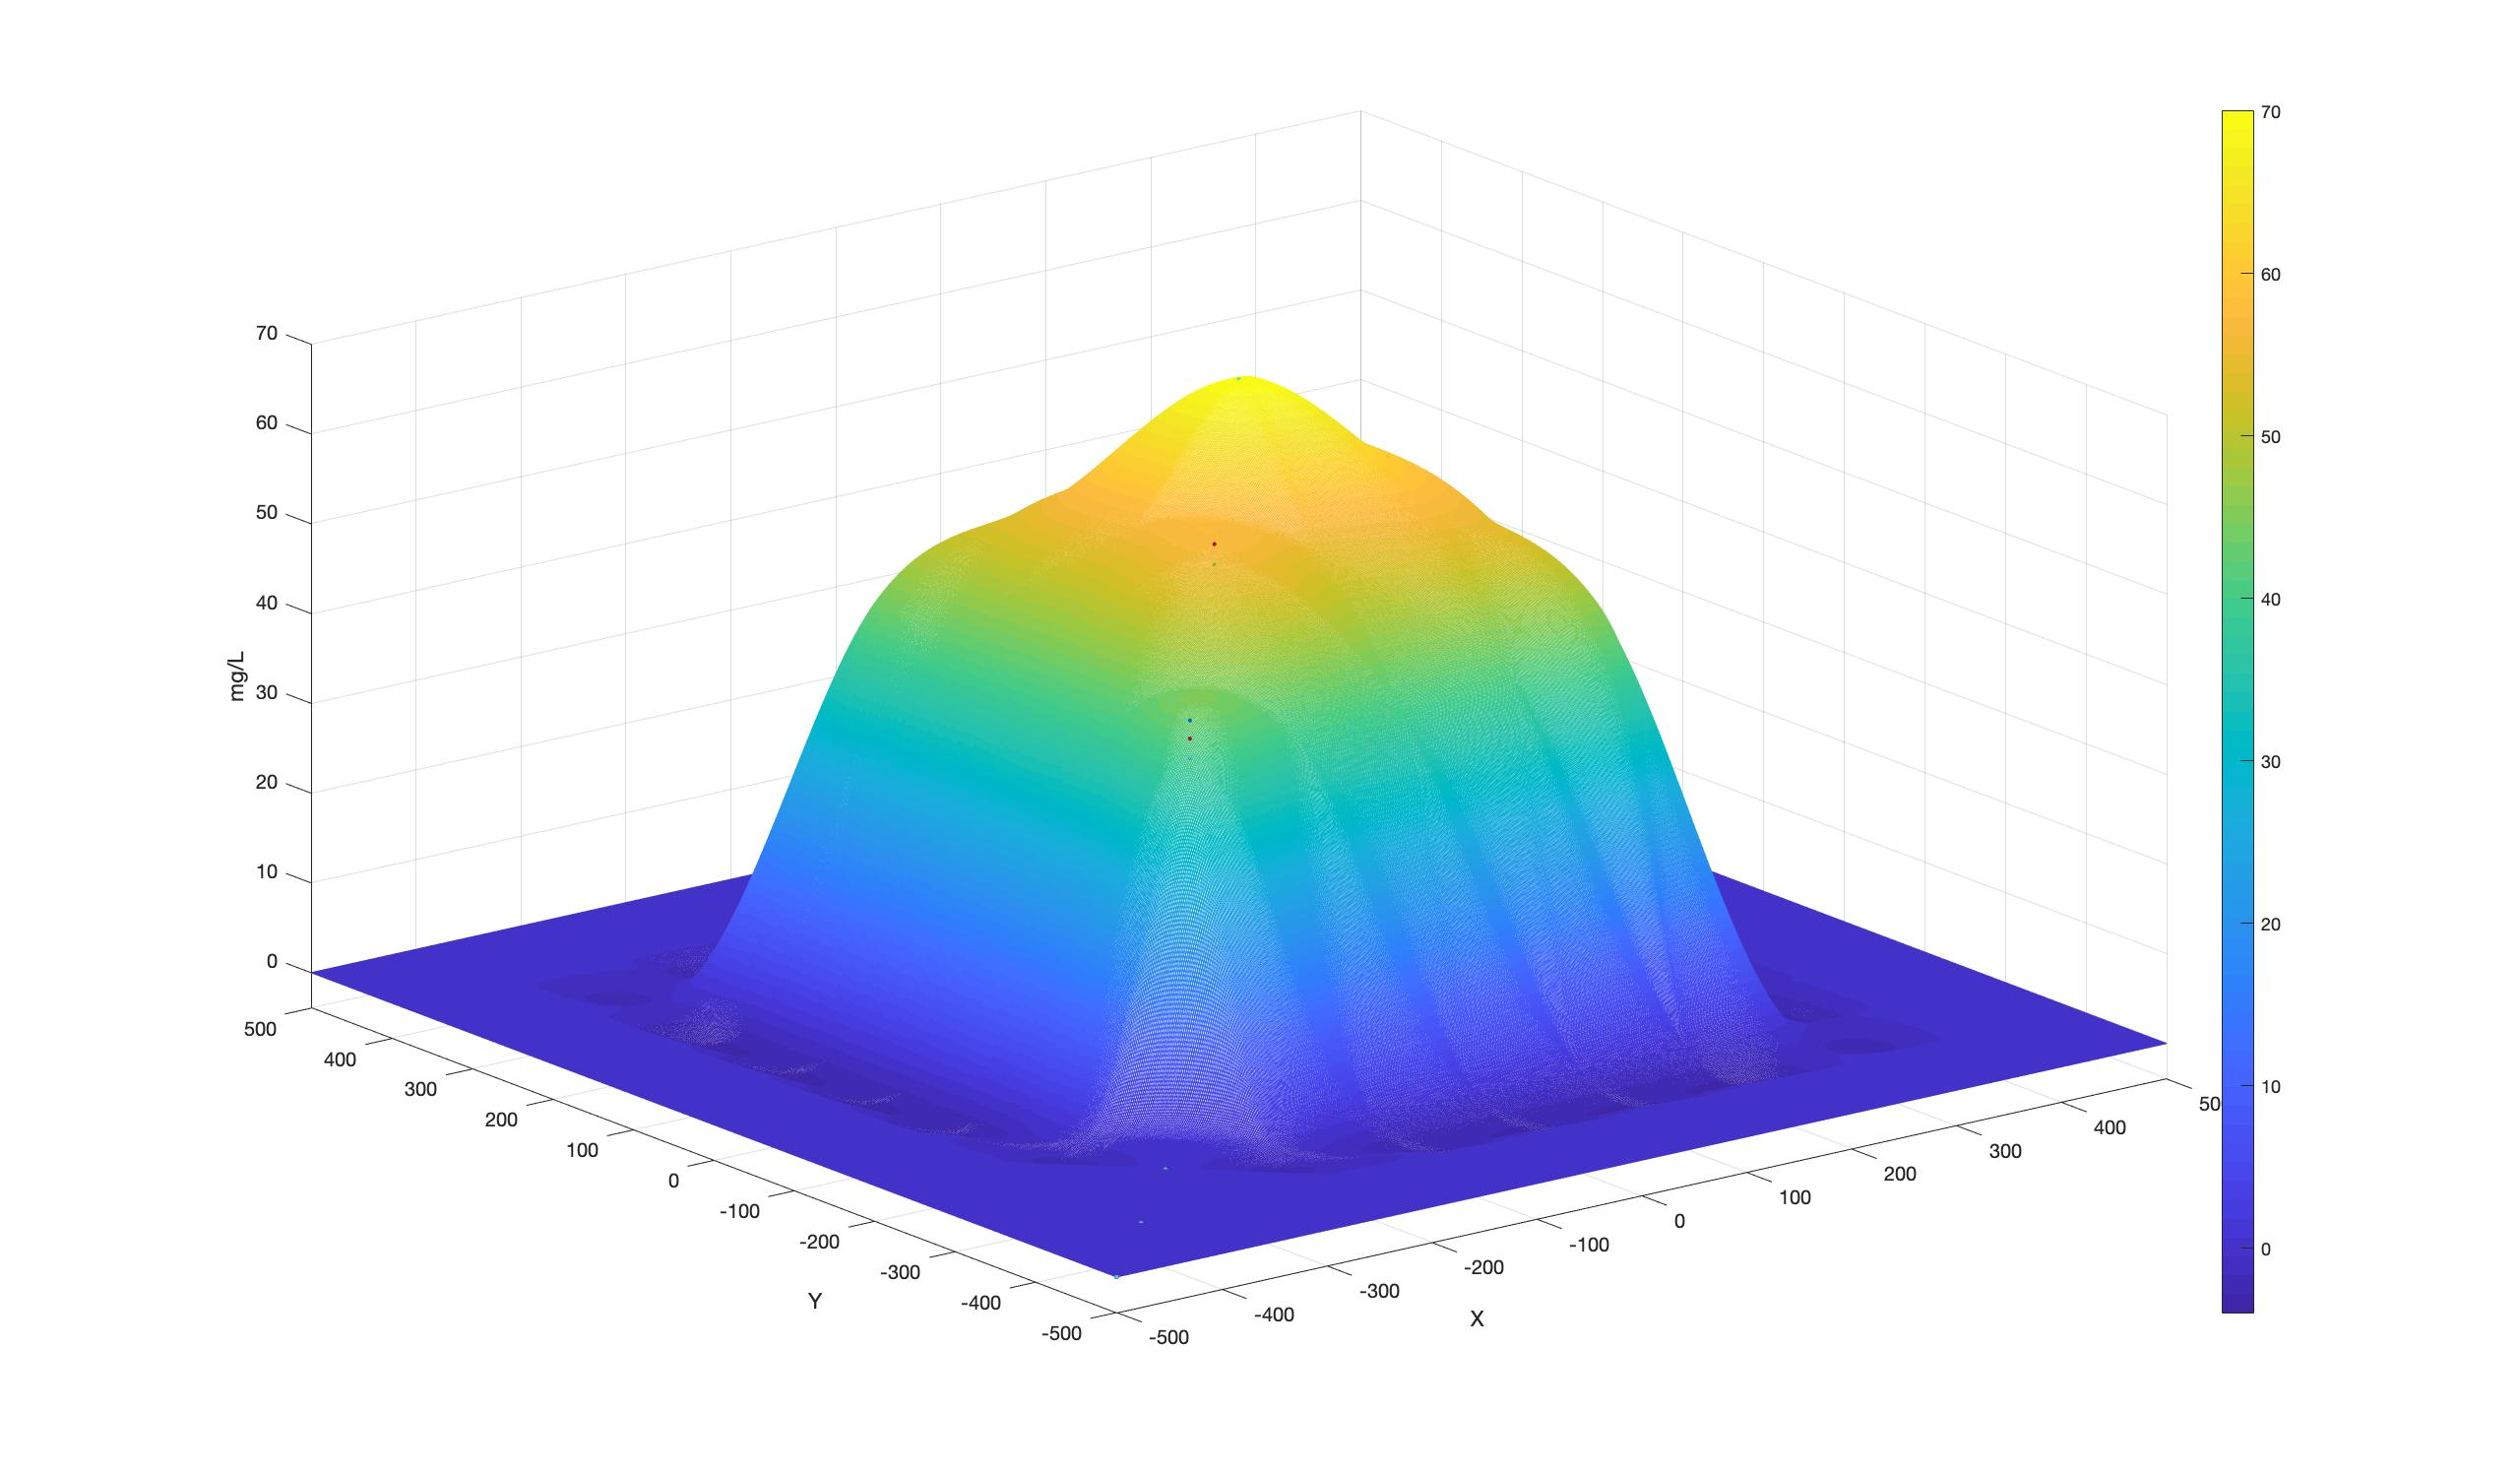
\includegraphics[width=.9\linewidth]{Images/Rec30_side.jpg}
  \subcaption{Rectangular 30x2.6}
\end{subfigure}
\caption{Visualisation of concentration (mg/l) for all nozzle shapes (sideview, 200x200 grid)}
\label{fig:side_concentratie}
\end{figure}

\begin{figure}[ht!]
\centering
\begin{subfigure}{.33\textwidth}
  \centering
  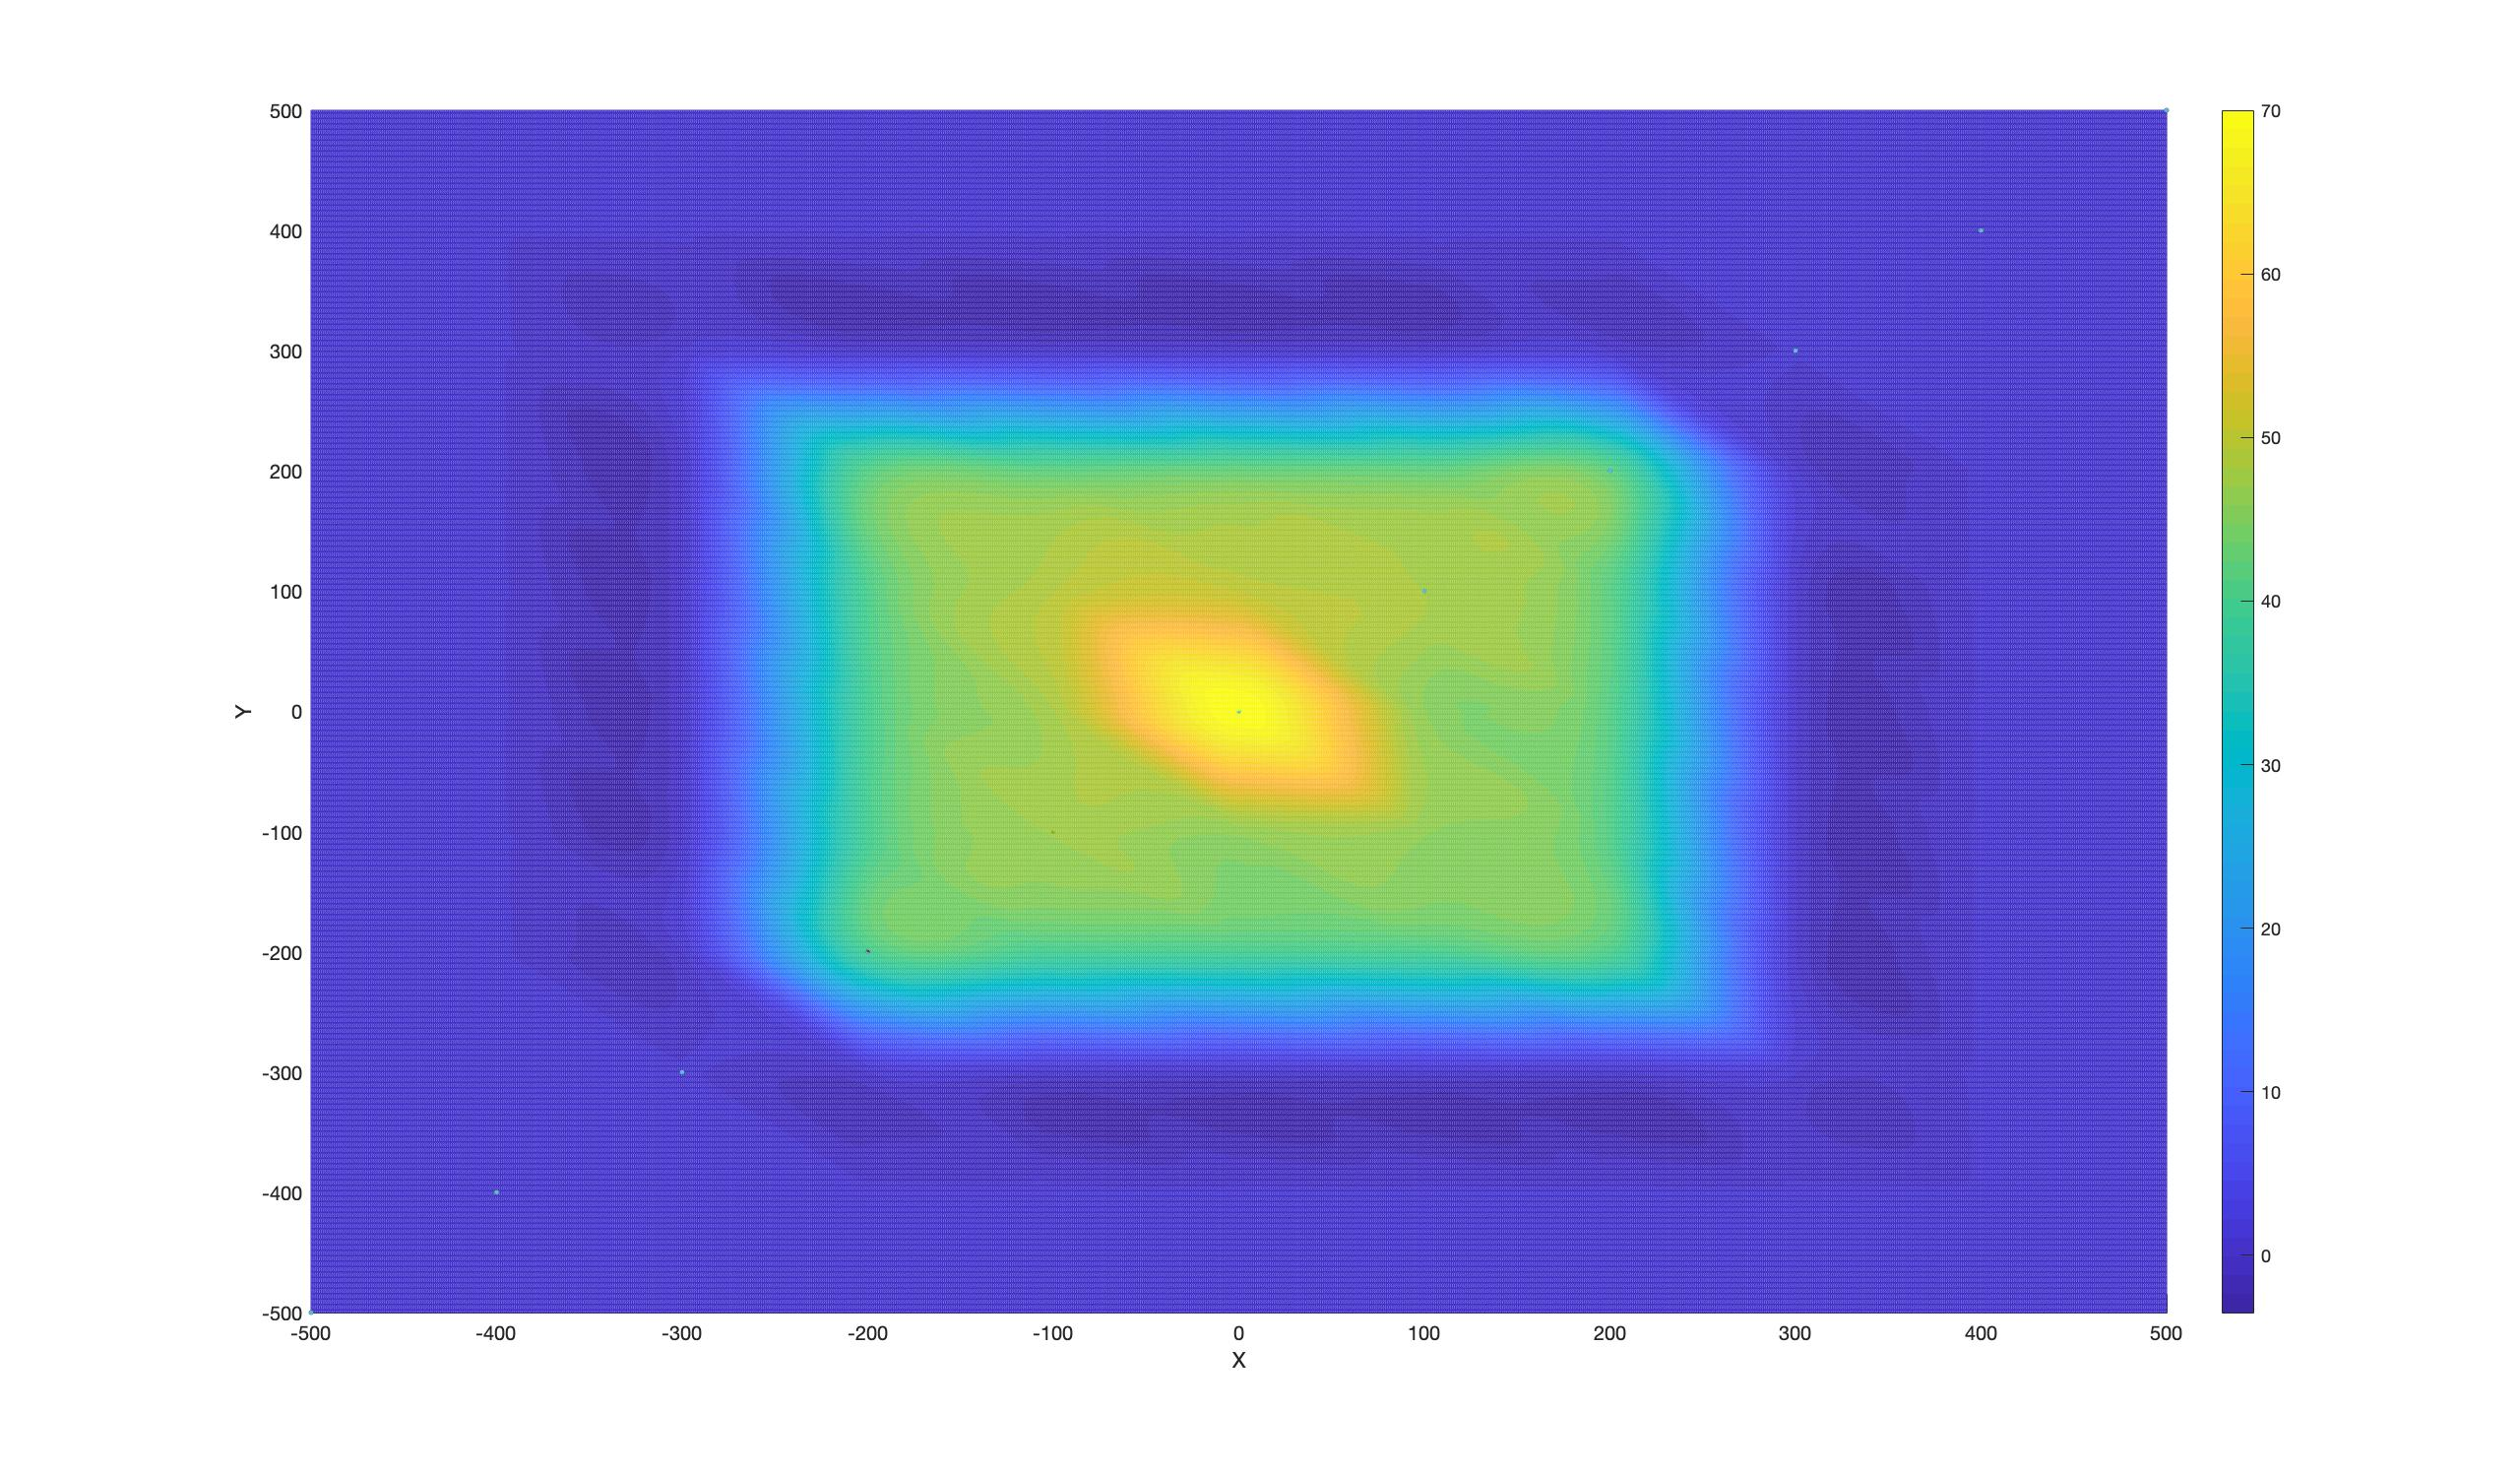
\includegraphics[width=.9\linewidth]{Images/Round_top.jpg}
  \subcaption{Round}
\end{subfigure}
\begin{subfigure}{.33\textwidth}
  \centering
  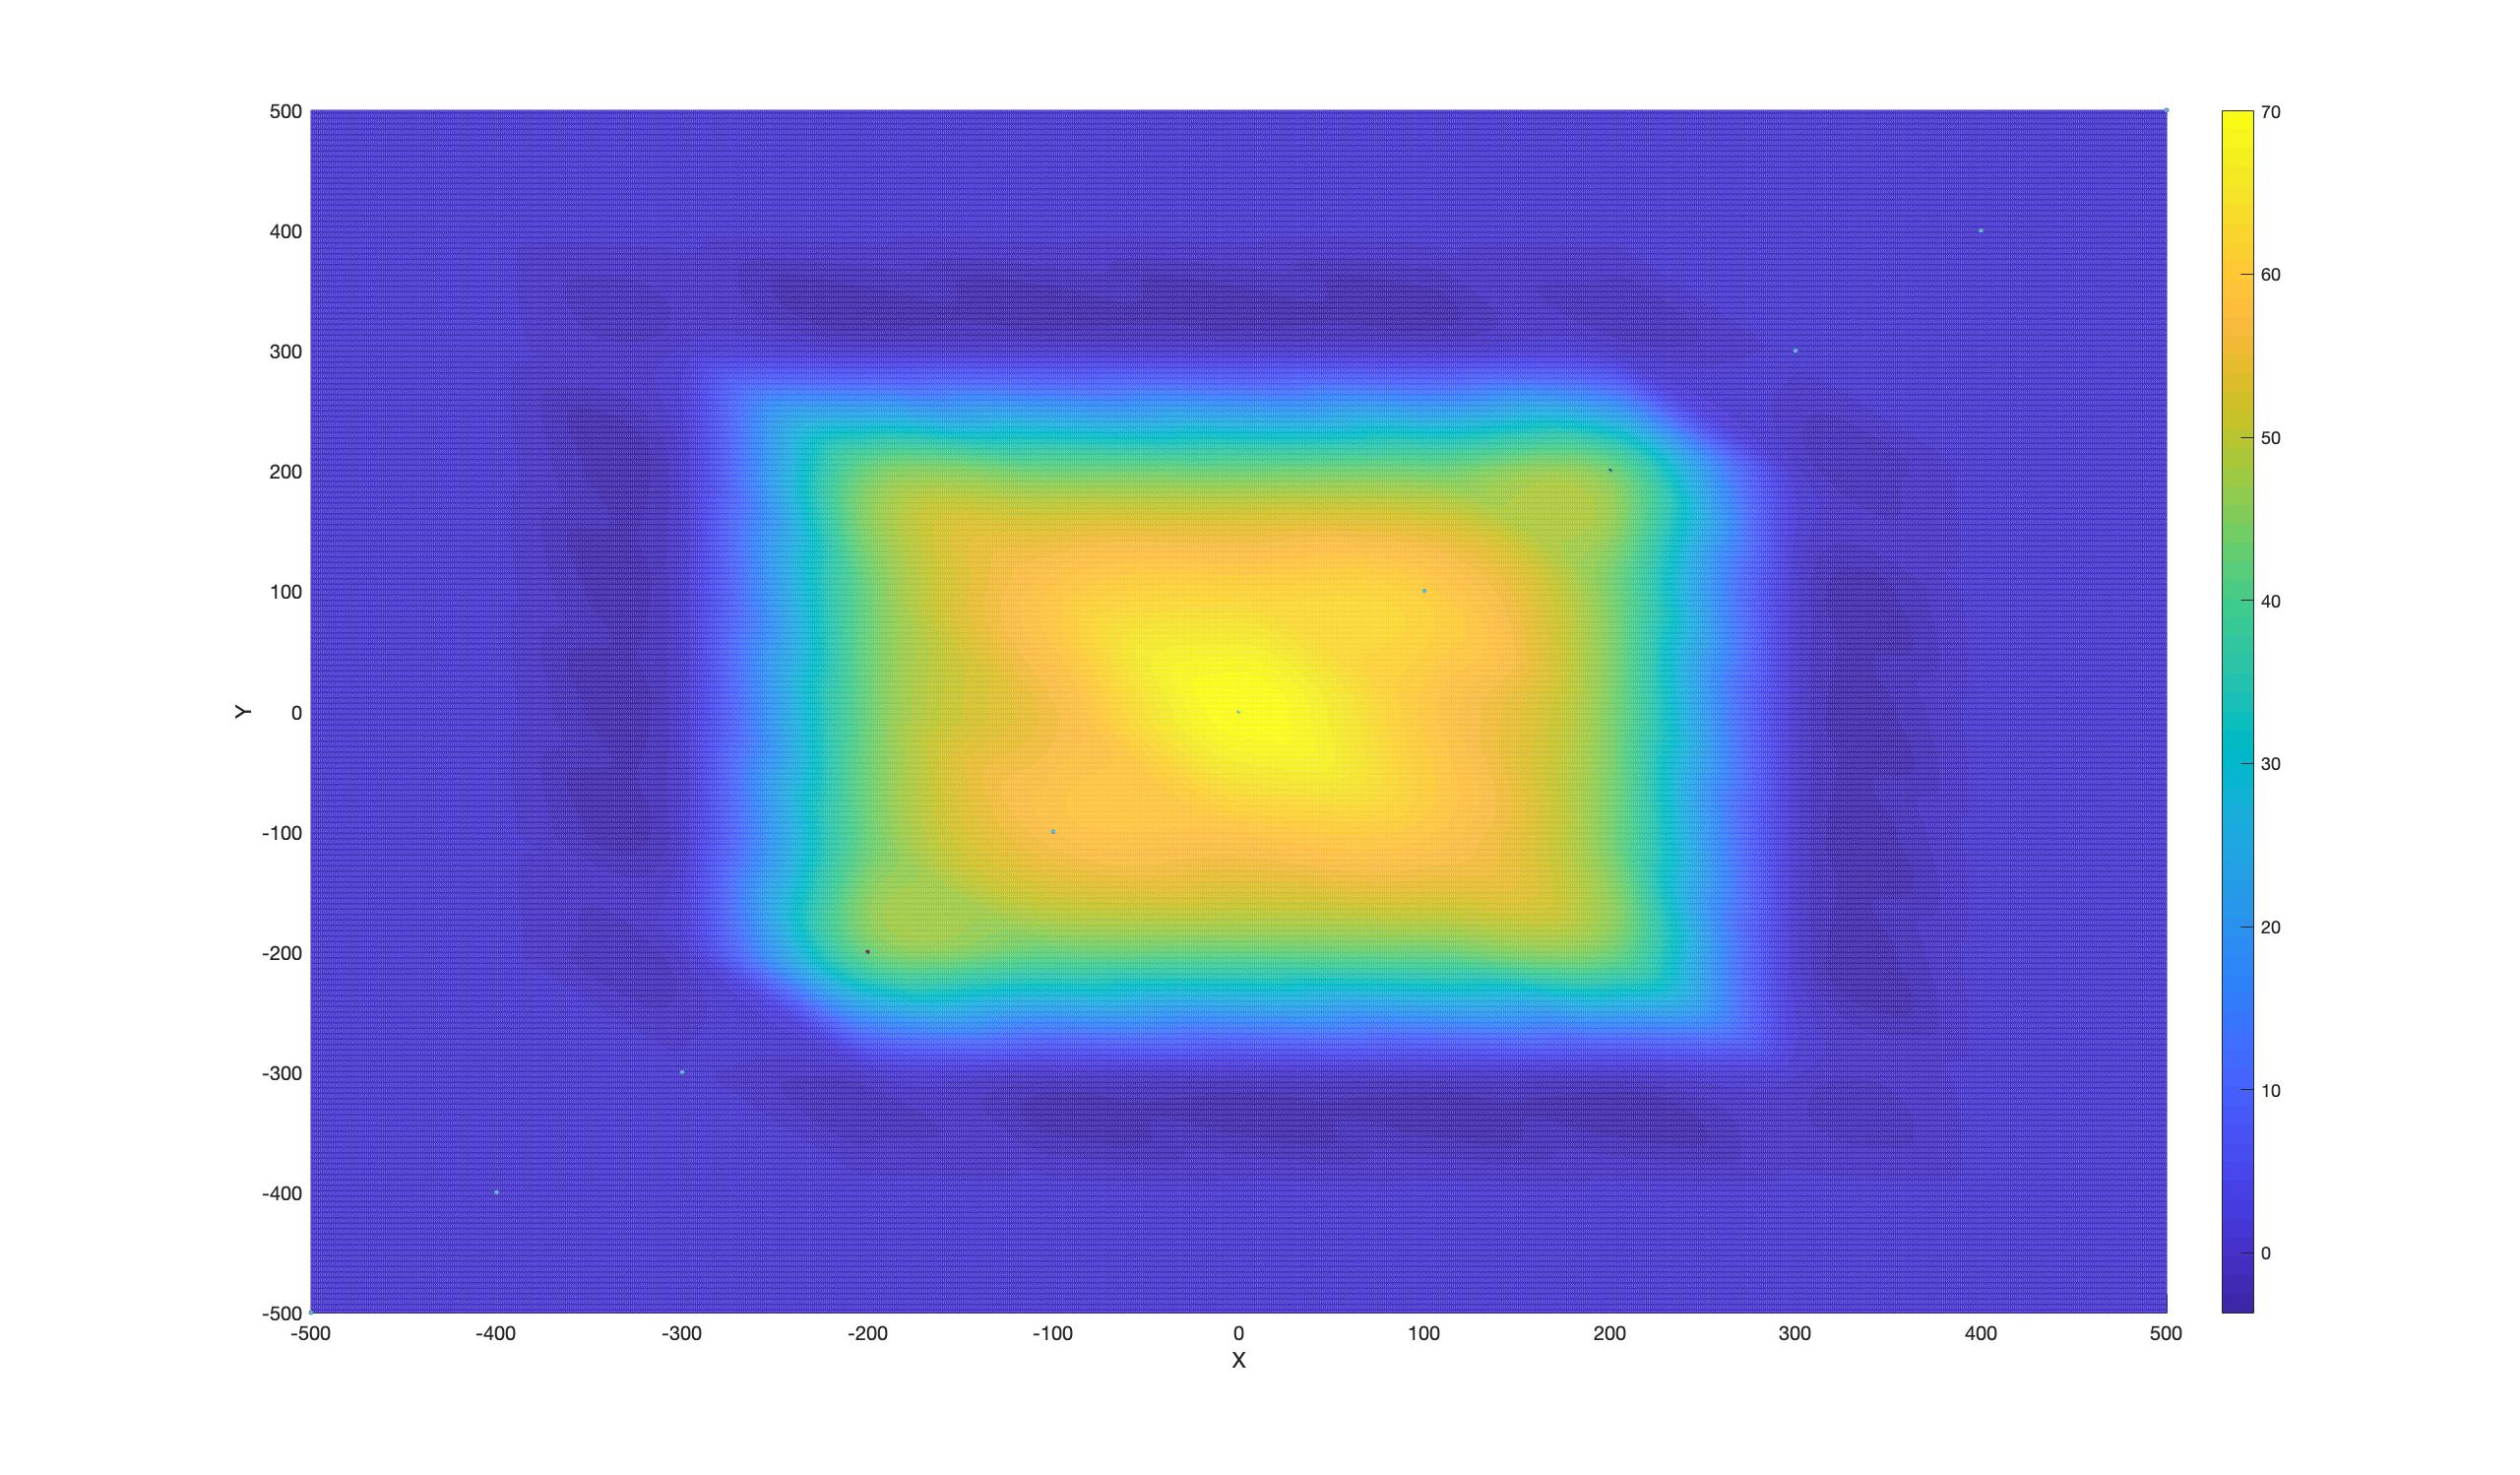
\includegraphics[width=.9\linewidth]{Images/Rec20_top.jpg}
  \subcaption{Rectangular 20x3.9}
\end{subfigure}
\begin{subfigure}{.33\textwidth}
  \centering
  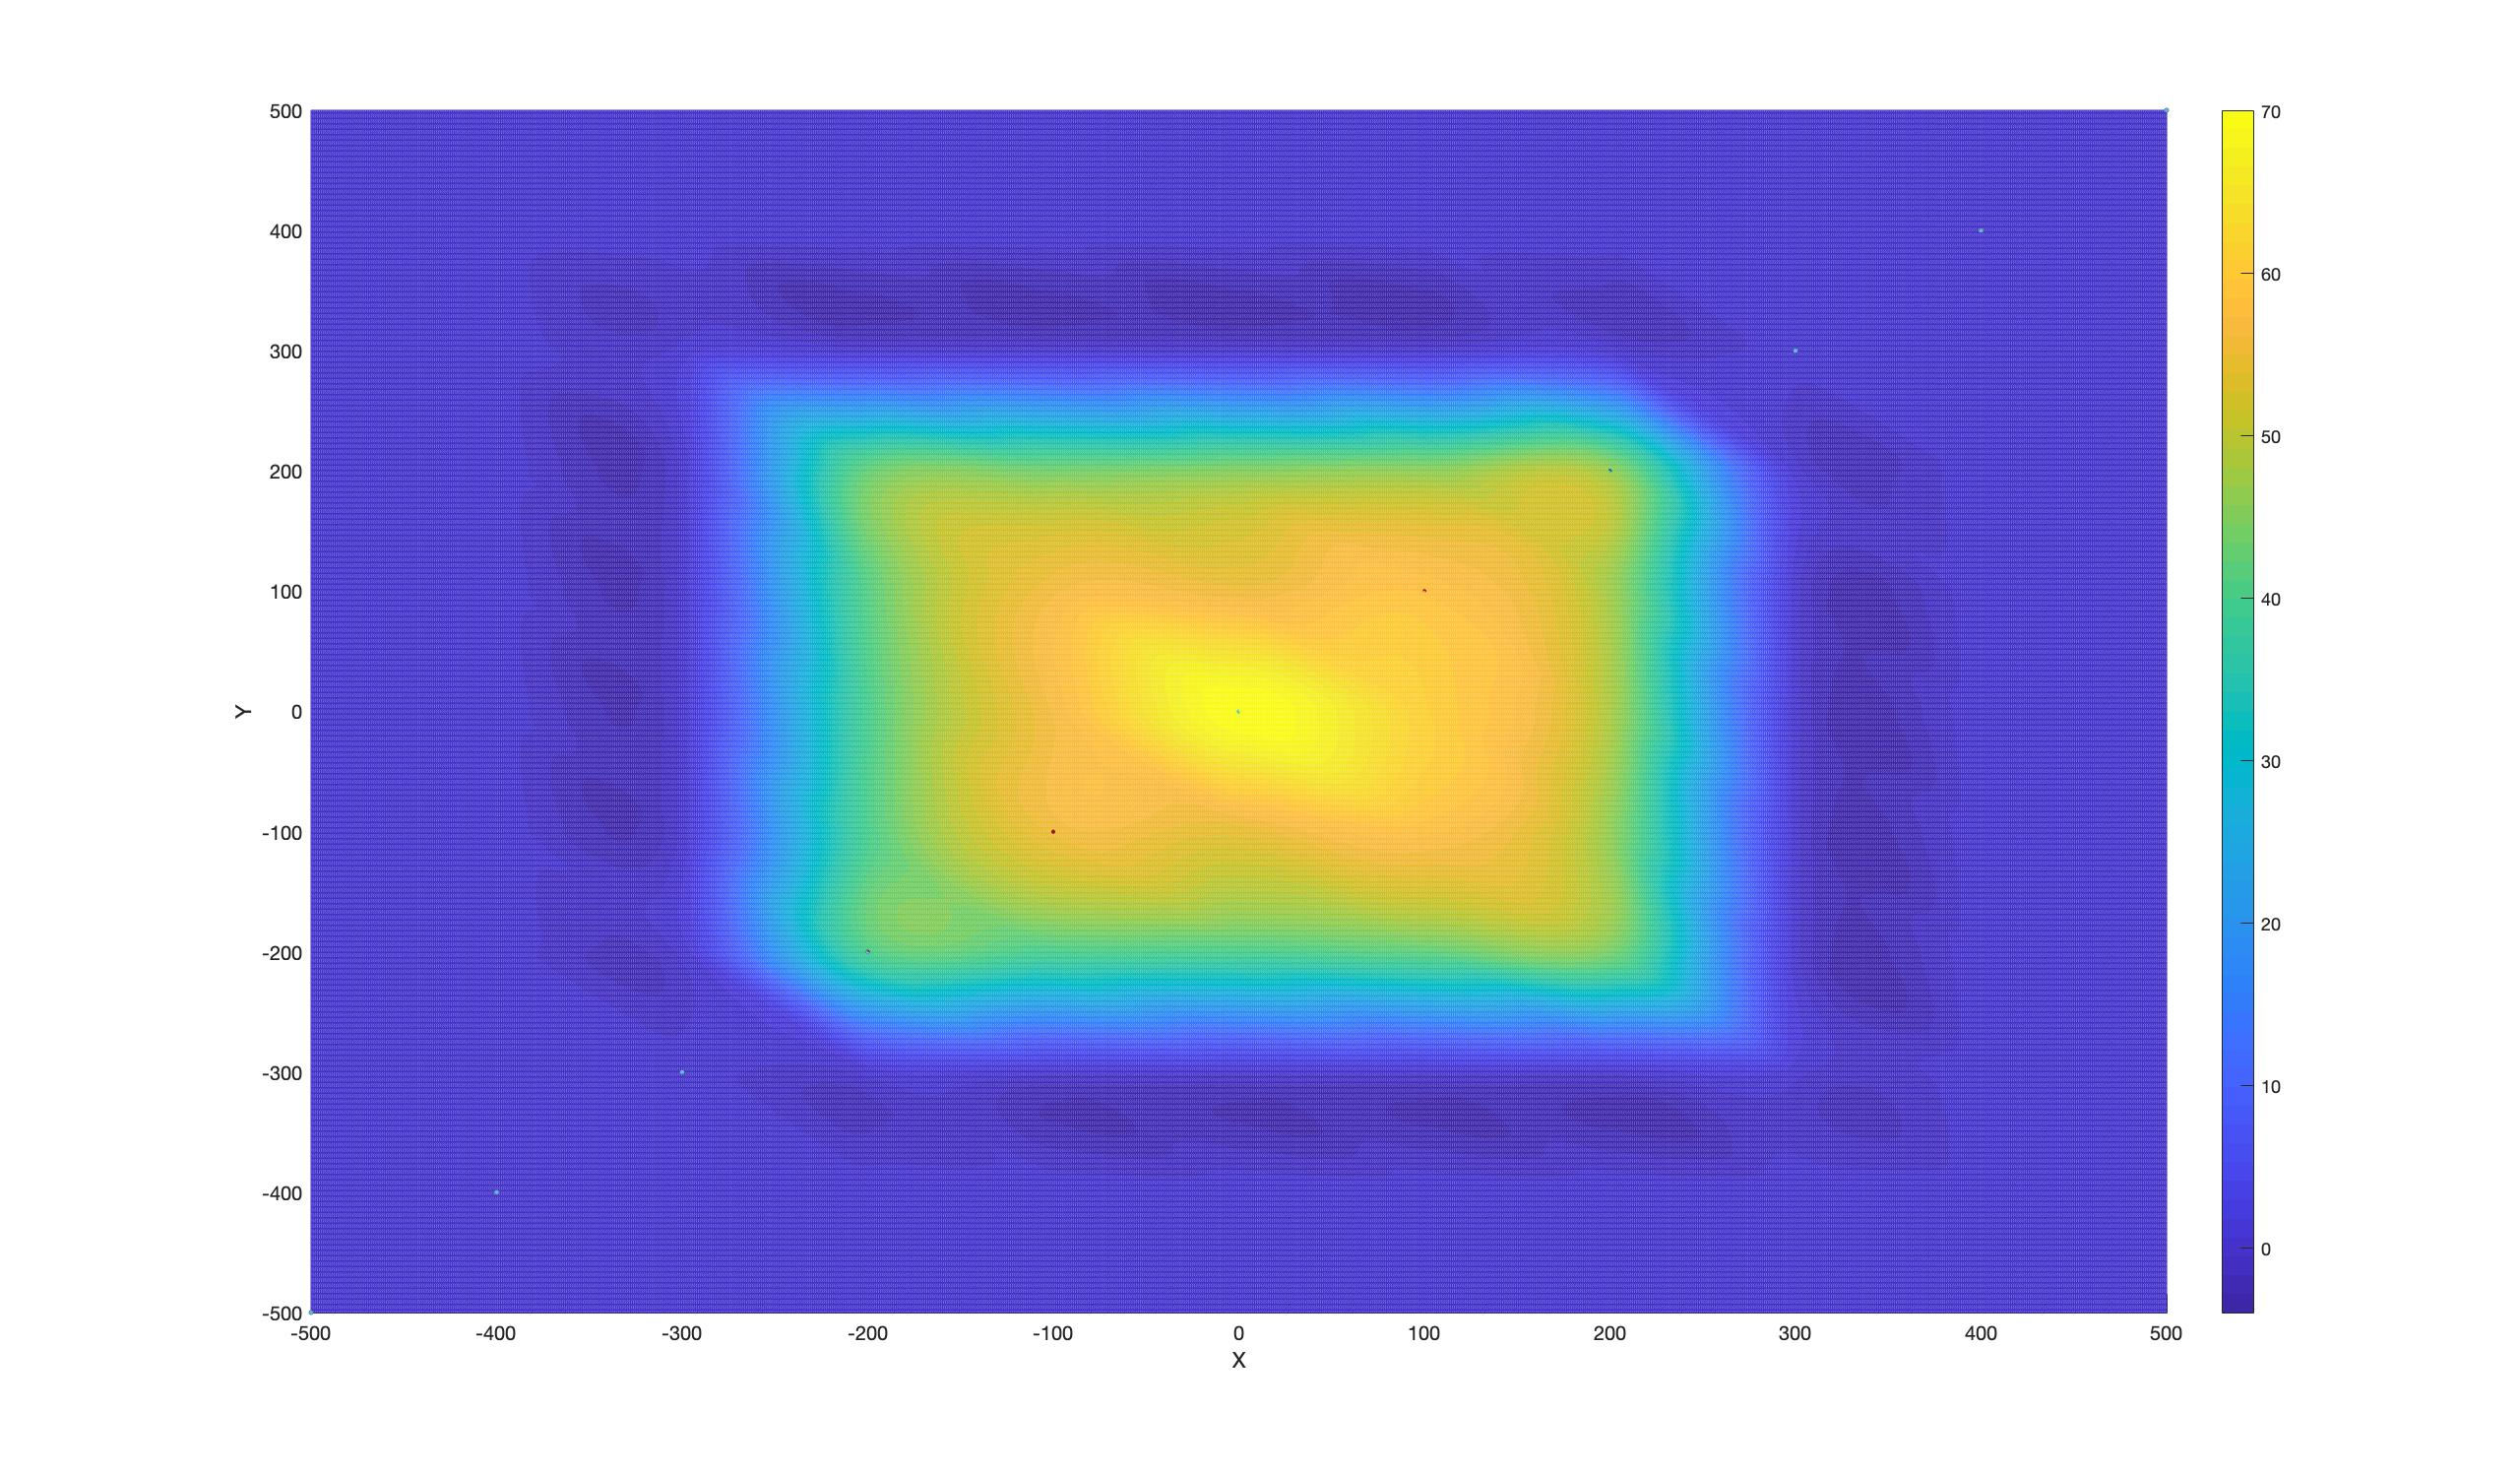
\includegraphics[width=.9\linewidth]{Images/Rec30_top.jpg}
  \subcaption{Rectangular 30x2.6}
\end{subfigure}
\caption{Visualisation of concentration (mg/l) for all nozzle shapes (topview, 200x200 grid)}
\label{fig:top_concentratie}
\end{figure}

\noindent The images in case of a round nozzle (figures \ref{fig:side_concentratie}a and \ref{fig:top_concentratie}a) show a lower concentration comparing to the rectangular nozzles. It should be noted that the middle value (70 mg/l) is a taken value and is not measured, therefore the result of the round nozzle shows a large peak in the middle point. Looking at the measurement points at 200mm radius (3, 6, 10, 12), which are also taken into account in the visualisation, remains almost the same in all three cases. The only noticeable difference is the increase of concentration for a radius < 200mm. It is assumed that the entrainment is better with a rectangular nozzle and so the plume has a smaller angle based on the concentration measurements.




%%%%%%%%%%%%%%%%%%%%%%%%%%%%%%%%%%%%%%%%%%%%%%%%%%%%%%%%%%%%%%%%%%%%%%%%%%%%%%%%%%%%%%%%%%%%%%%%%%%%%%%%%%%%%%%%%%%%%%%%%%%%%%%%%%%%%%%%%%%%%%%%%%%%%%%%%%%%%%%%%%%%%%%%%%%%%%%%%%%%%%%%%%%%%%%%%%%%%%%%%%%%%%%%%%%%%%%%%%%%%%%%%%%%%%%%

\section{Angle measurements}
Showing an increase of concentration in case of a rectangular nozzle shape should connect to less entrainment with the surrounding ambient water. A steeper angle of the plume should be measured in this case, which is investigated in this section. The determination of the entrainment angles based on a contour trendlines is shown in appendix \ref{app:Angles}.


\subsection{Entrainment angles}
In a total of 45 experiments, the entrainment angle is measured. It was not possible to capture the total height in the camera frame. Therefore the angle was measured from the moment the plume entered the camera frame until it reached the bottom plate. By following the contour the plume and creating two trendlines (left- and right contour plume), the angle is calculated between the two trendlines. An example is shown in figure \ref{fig:example}. All snapshots of the plumes, at the point where the angles are measured, are shown in appendix \ref{app:Angles}. An overview of all calculated angles is shown in table \ref{tab:angles}.

\begin{figure}[ht!]
    \centering
    \includegraphics[width =0.6\textwidth]{Textfiles/Round_1_example.png}
    \caption{Determination of contour trendlines for test Round 1}
    \label{fig:example}
\end{figure}


\begin{table}[ht!]
\centering
\begin{adjustbox}{max width = 0.6\linewidth}
\begin{tabular}{lll|c|c|c|c|c|}
\cline{1-2} \cline{4-5} \cline{7-8}
\multicolumn{2}{|c|}{\textbf{Round}} &  & \multicolumn{2}{c|}{\textbf{Rectangular 20x3.9mm}} &  & \multicolumn{2}{c|}{\textbf{Rectangular 30x2.6mm}} \\ \cline{1-2} \cline{4-5} \cline{7-8} 
\multicolumn{1}{|c|}{\textbf{Test \#}} & \multicolumn{1}{c|}{\textbf{Angle $(^\circ)$}} &  & \textbf{Test \#} & \textbf{Angle $(^\circ)$} &  & \textbf{Test \#} & \textbf{Angle $(^\circ)$} \\ \cline{1-2} \cline{4-5} \cline{7-8}
\multicolumn{1}{|c|}{1} & \multicolumn{1}{c|}{25.17} &  & 1 & 18.77 &  & 1 & 22.47 \\ \cline{1-2} \cline{4-5} \cline{7-8} 
\multicolumn{1}{|c|}{2} & \multicolumn{1}{c|}{29.56} &  & 2 & 24.60 &  & 2 & 23.26 \\ \cline{1-2} \cline{4-5} \cline{7-8} 
\multicolumn{1}{|c|}{3} & \multicolumn{1}{c|}{26.27} &  & 3 & 24.10 &  & 3 & 17.77 \\ \cline{1-2} \cline{4-5} \cline{7-8} 
\multicolumn{1}{|c|}{4} & \multicolumn{1}{c|}{25.81} &  & 4 & 20.08 &  & 4 & 22.70 \\ \cline{1-2} \cline{4-5} \cline{7-8} 
\multicolumn{1}{|c|}{5} & \multicolumn{1}{c|}{24.97} &  & 5 & 20.86 &  & 5 & 20.14 \\ \cline{1-2} \cline{4-5} \cline{7-8} 
 &  &  & 6 & 22.51 &  & 6 & 23.13 \\ \cline{4-5} \cline{7-8} 
 &  &  & 7 & 21.93 &  & 7 & 19.44 \\ \cline{4-5} \cline{7-8} 
 &  &  & 8 & 23.73 &  & 8 & 23.76 \\ \cline{4-5} \cline{7-8} 
 &  &  & 9 & 20.75 &  & 9 & 20.85 \\ \cline{4-5} \cline{7-8} 
 &  &  & 10 & 22.87 &  & 10 & 20.38 \\ \cline{4-5} \cline{7-8} 
 &  &  & 11 & 27.07 &  & 11 & 19.48 \\ \cline{4-5} \cline{7-8} 
 &  &  & 12 & 22.08 &  & 12 & 23.80 \\ \cline{4-5} \cline{7-8} 
 &  &  & 13 & 20.55 &  & 13 & 22.96 \\ \cline{4-5} \cline{7-8} 
 &  &  & 14 & 25.23 &  & 14 & 18.89 \\ \cline{4-5} \cline{7-8} 
 &  &  & 15 & 27.19 &  & 15 & 24.08 \\ \cline{4-5} \cline{7-8} 
 &  &  & 16 & 25.16 &  & 16 & 19.47 \\ \cline{4-5} \cline{7-8} 
 &  &  & 17 & 21.09 &  & 17 & 19.33 \\ \cline{4-5} \cline{7-8} 
 &  &  & 18 & 28.14 &  & 18 & 21.56 \\ \cline{4-5} \cline{7-8} 
 &  &  & 19 & 21.77 &  & 19 & 23.24 \\ \cline{4-5} \cline{7-8} 
 &  &  & 20 & 23.39 &  & 20 & 20.58 \\ \cline{4-5} \cline{7-8} 
\end{tabular}
\end{adjustbox}
\caption{Calculated angles for each nozzle. Note that for the both rectangular nozzles experiments 11-20 the nozzle is turned 90 degrees}
\label{tab:angles}
\end{table}

\noindent Comparing the angles, lower angles are found in case of a rectangular nozzle. Looking at table \ref{tab:average_angles}, which shows the average calculated angle with error (which should be < 1$^\circ$), it shows that the angle is indeed lower in case of the rectangular nozzles. The average angle is reduced in a range of 8.3\% - 19\% based of the measured angle experiment.

\begin{table}[ht!]
\centering
\begin{adjustbox}{max width = 0.8\textwidth}
\begin{tabular}{|c|c|c|}
\hline
\textbf{Nozzle shape} & \textbf{Average angle $(^\circ)$} & \textbf{Error $(^\circ)$} \\ \hline
Round & 26.36 & 0.75 \\ \hline
Rectangular 20x3.9 - 3.9 & 22.02 & 0.58 \\ \hline
Rectangular 20x3.9 - 20 & 24.17 & 0.83 \\ \hline
Rectangular 30x2.6 - 2.6 & 21.39 & 0.59 \\ \hline
Rectangular 30x2.6 - 30 & 21.34 & 0.61 \\ \hline
\end{tabular}
\end{adjustbox}
\caption{Averaged angles and error for each nozzle shape. The last number (- xx) for the rectangular nozzles shows the side which faced the camera}
\label{tab:average_angles}
\end{table}

\noindent In order to test if the aspect ratio has effect on the entrainment angle, the nozzle in case of rectangular shape is turned 90 degrees (experiments 11-20). Based on the experiments, is shows that if the aspect ratio increases of the rectangular nozzle, the entrainment angles decrease in both orientations and even become nearly constant in the case of the 30x2.6mm nozzle. It should be noted that the rectangular shapes show more fluctuation between measurements, but definitely decrease the averaged entrainment angle of the plume. The finding of the lower entrainment angle connects with the denser concentration near the middle point which is found in the concentration measurements.


\subsection{Entrainment coefficient}
In order to determine the entrainment coefficient, the literature from chapter \ref{ch:Analytical} is used. Here we combine the knowledge of the reference frame from figure \ref{fig:round_plume} where there is a difference between the velocity width and concentration width, which is related to the concentration to velocity ratio $(\lambda_r)$. In section \ref{sec:summary_entrainment} the entrainment coefficients $(\alpha_G)$ and concentration to velocity ratio are shown in case of round jets and plumes, and plane jets ans plumes. Knowing that is assumed that the plume spreads linearly, the velocity width (b) was denoted as $b = \beta_G * z$. Relating this spreading rate back to the measured angles, which measure the plume width, we can find the velocity width with formula \ref{for:gam} for all 4 cases. Table \ref{tab:b} shows the calculated b and $\beta$ in all cases. The measured half angle is denoted as $\gamma$, where z is the height.


\begin{equation}
    \centering
    tan (\gamma) = \frac{\lambda_r * b}{z}
    \label{for:gam}
\end{equation}


\begin{table}[ht!]
\centering
\begin{adjustbox}{max width =\textwidth}
\begin{tabular}{|c|c|c|c|c|c|}
\hline
 & \textbf{Round} & \textbf{Rectangular 20x3.9 - 3.9} & \textbf{Rectangular 20x3.9 - 20} & \textbf{Rectangular 30x2.6 - 2.6} & \textbf{Rectangular 30x2.6 - 30} \\ \hline
\textbf{Angle} $\bm{(\gamma)}$ & 13.18 & 11.01 & 12.085 & 10.695 & 10.67 \\ \hline
\textbf{Concentration width $\bm{(\lambda_r b)}$} & 0.3712 & 0.3084 & 0.3394 & 0.2993 & 0.2986 \\ \hline
\textbf{Velocity width} $\bm{(b)}$ & 0.3119 & 0.2284 & 0.2514 & 0.2217 & 0.2212 \\ \hline
\textbf{Spreading rate} $\bm{(\beta_G)}$ & 0.1968 & 0.1441 & 0.1586 & 0.1399 & 0.1396 \\ \hline
\end{tabular}
\end{adjustbox}
\caption{Calculated concentration width, velocity width and spreading rated bases on measured angles}
\label{tab:b}
\end{table}

\noindent Now that the spreading rate is known, the entrainment coefficient can be determined using the relations found in chapter \ref{ch:Analytical}, which is summarized in section \ref{sec:summary_entrainment}. Table \ref{tab:entrainment_coefficients} show the calculated entrainment coefficients in case of a jet and a plume, for all angles measured during the experiment.


\begin{table}[ht!]
\centering
\begin{adjustbox}{max width = \textwidth}
\begin{tabular}{|c|c|c|c|c|c|}
\hline
\multicolumn{1}{|l|}{} & \textbf{Round} & \textbf{Rectangular 20x3.9 - 3.9} & \textbf{Rectangular 20x3.9 - 20} & \textbf{Rectangular 30x2.6 - 2.6} & \textbf{Rectangular 30x2.6 - 30} \\ \hline
\bm{$\alpha_G - jet$} & 0.0984 & 0.0639 & 0.0703 & 0.0620 & 0.0618 \\ \hline
\bm{$\alpha_G - plume$} & 0.1640 & 0.1277 & 0.1406 & 0.1240 & 0.1237 \\ \hline
\end{tabular}
\end{adjustbox}
\caption{Calculated entrainment coefficients $(\alpha_G)$ by using table \ref{tab:alpha_lambda}}
\label{tab:entrainment_coefficients}
\end{table}

\noindent As determined before, by finding a smaller angle in case of a rectangular nozzle, the entrainment in this case is better compared to a round nozzle. Even that the methods do determine the entrainment coefficient is different in case of round jets and planes and plane jets and planes, the rectangular (plane) nozzles show a lower entrainment coefficient, which relates to less entrainment with the ambient water. In case of a jet, the entrainment coefficient is reduced with a range of 28.6\% - 37.2\%. In case of a plume, the entrainment coefficient is reduced with a range of 14.3\% - 24.6\%. Connecting this to the reduction found for the averaged angles, it is shown that a relative small angle reduction (8.3\%) decreases the entrainment coefficient, both for jets and plumes, with >14\%. It is also visible that with a larger decrease in angle, the entrainment coefficient also decreases further and follows the trend of the decreasing line of the angle. An overview of the decrease of all angles and entrainment coefficients is shown in figure \ref{fig:overview_angle_entrainment}. The effect of the entrainment coefficient combined with crossflow is further collaborated in chapter \ref{CH:model}. 



\begin{figure}
    \centering
    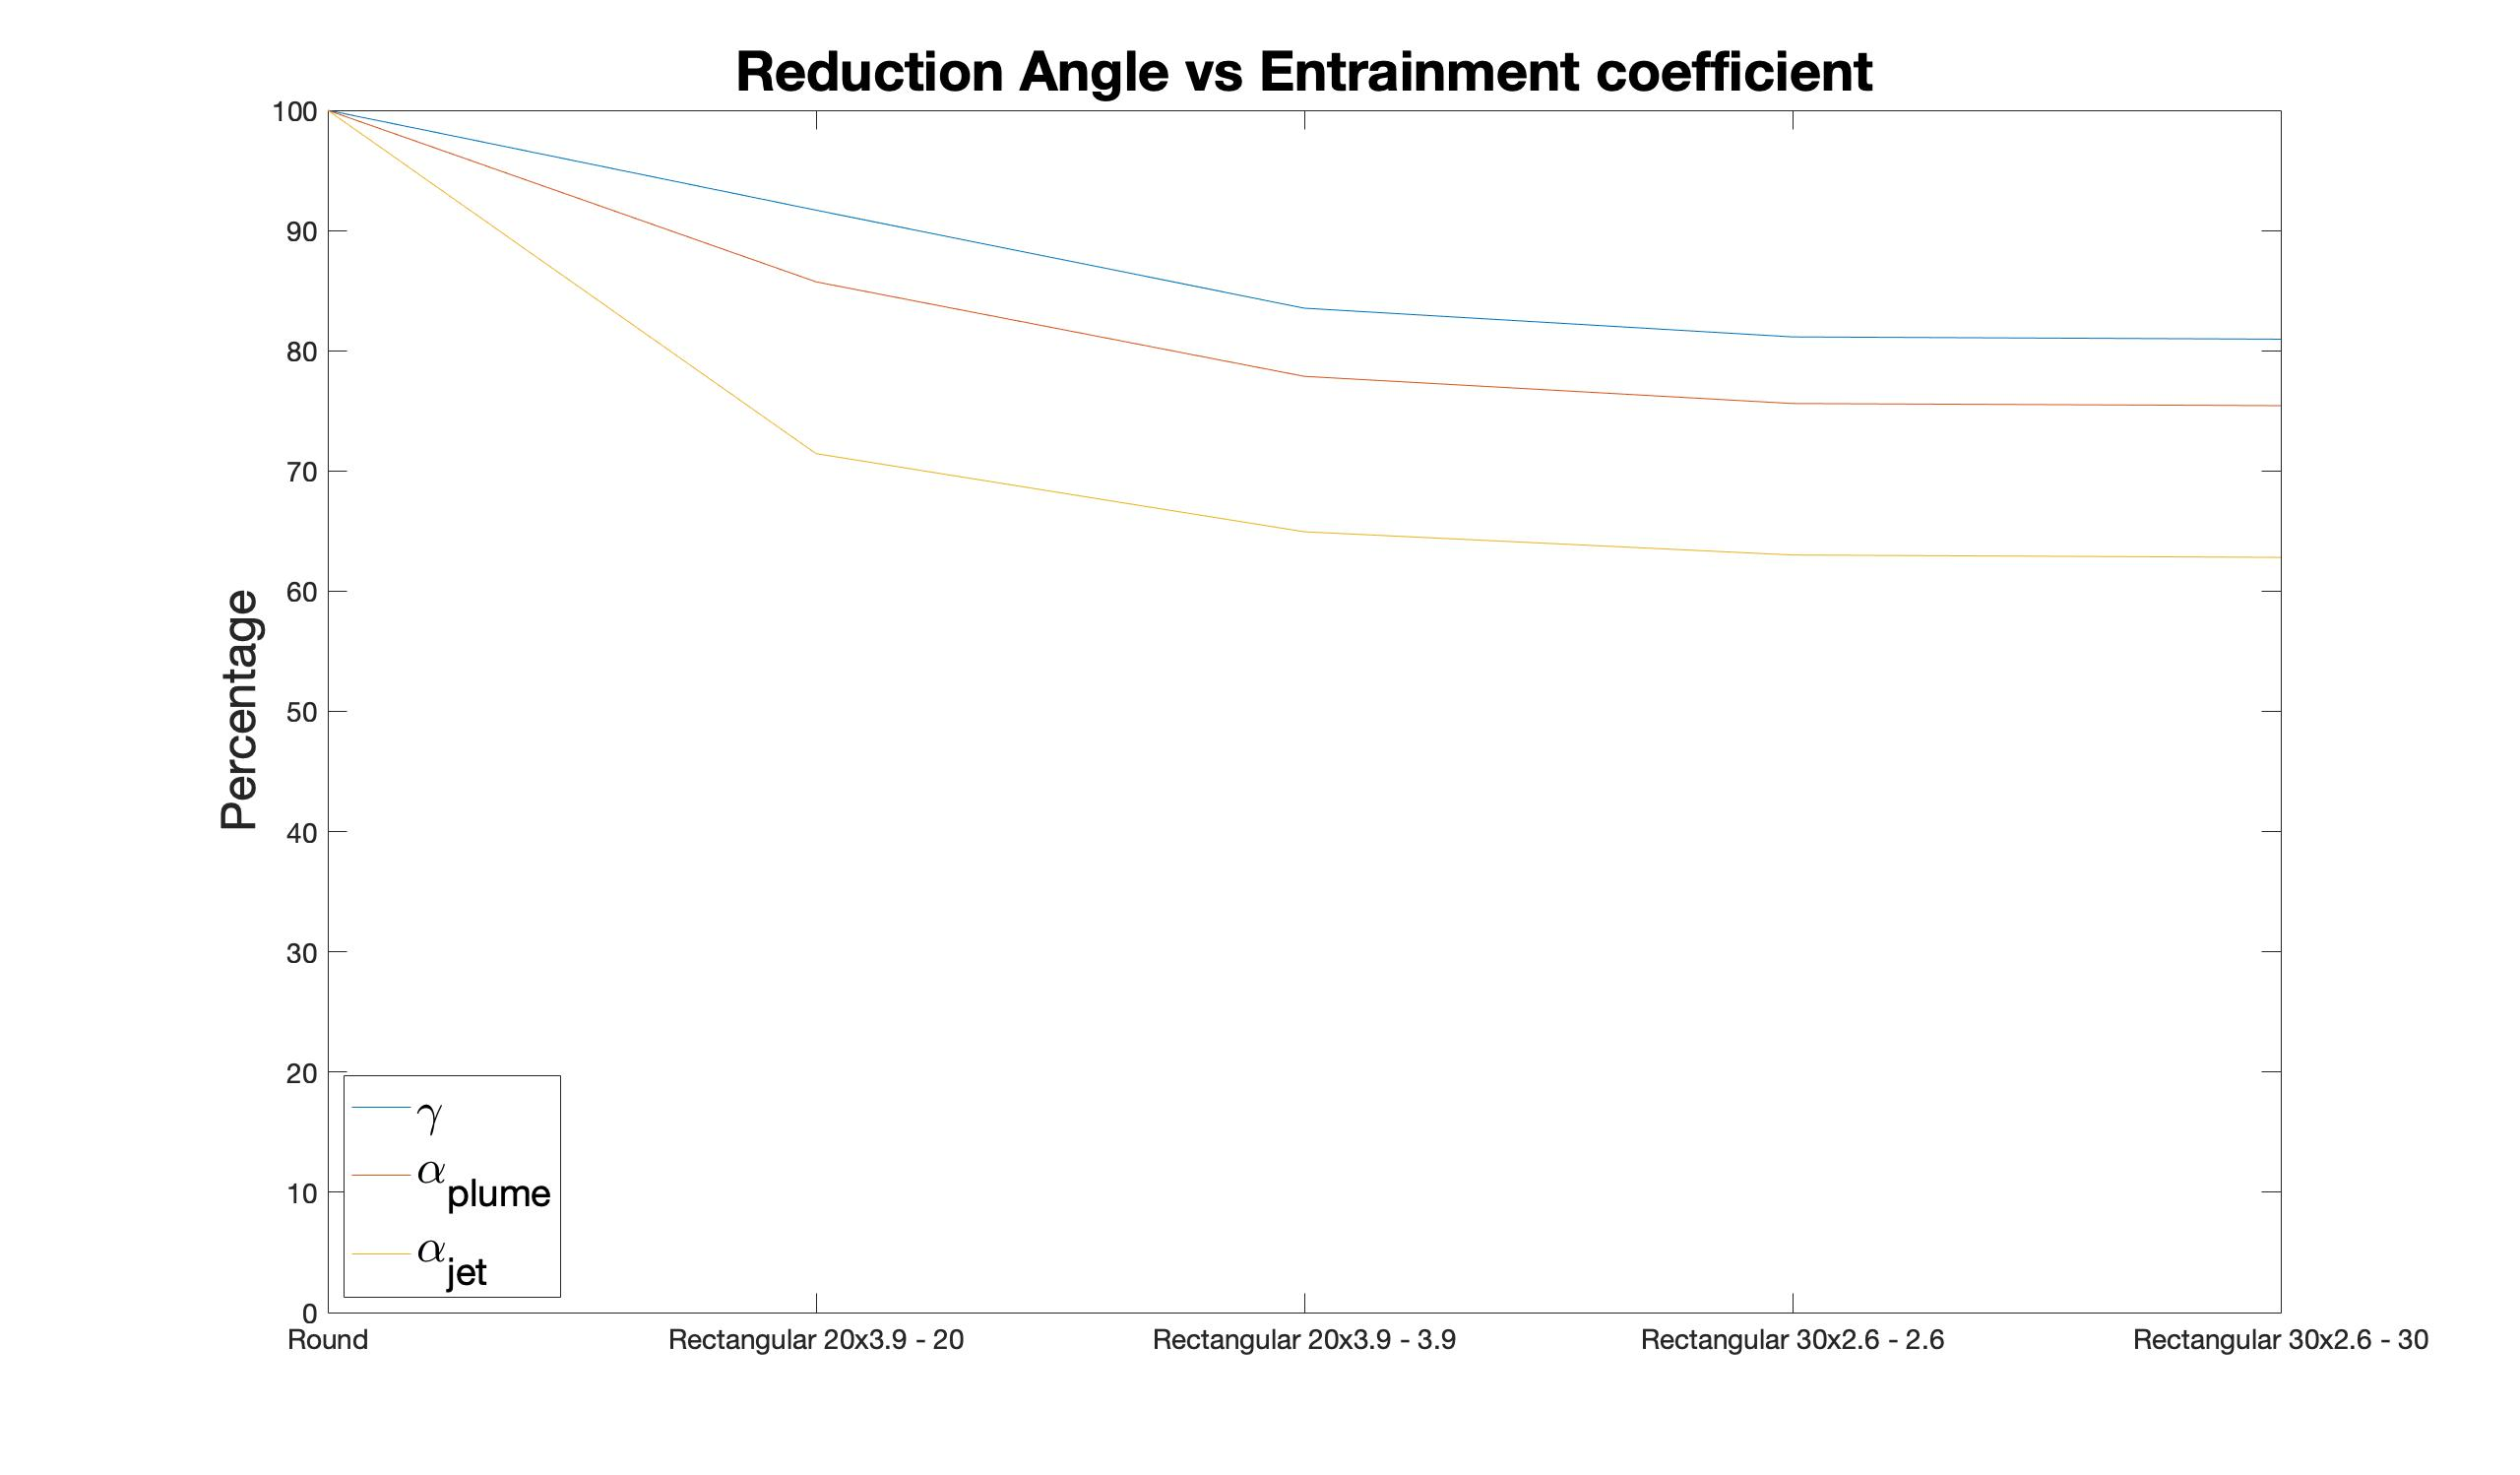
\includegraphics[width = 0.8\textwidth] {Images/Reduction_graph.jpg}
    \caption{Overview reduction of measured angle $(\gamma)$ and entrainment coefficient for jet $(\alpha_{jet})$ and plume $(\alpha_{plume})$}
    \label{fig:overview_angle_entrainment}
\end{figure}






\newpage
\subsection{Travel time}
%uitleg frame (bovenkant tot rand plaat)


\begin{figure}[ht!]
    \centering
    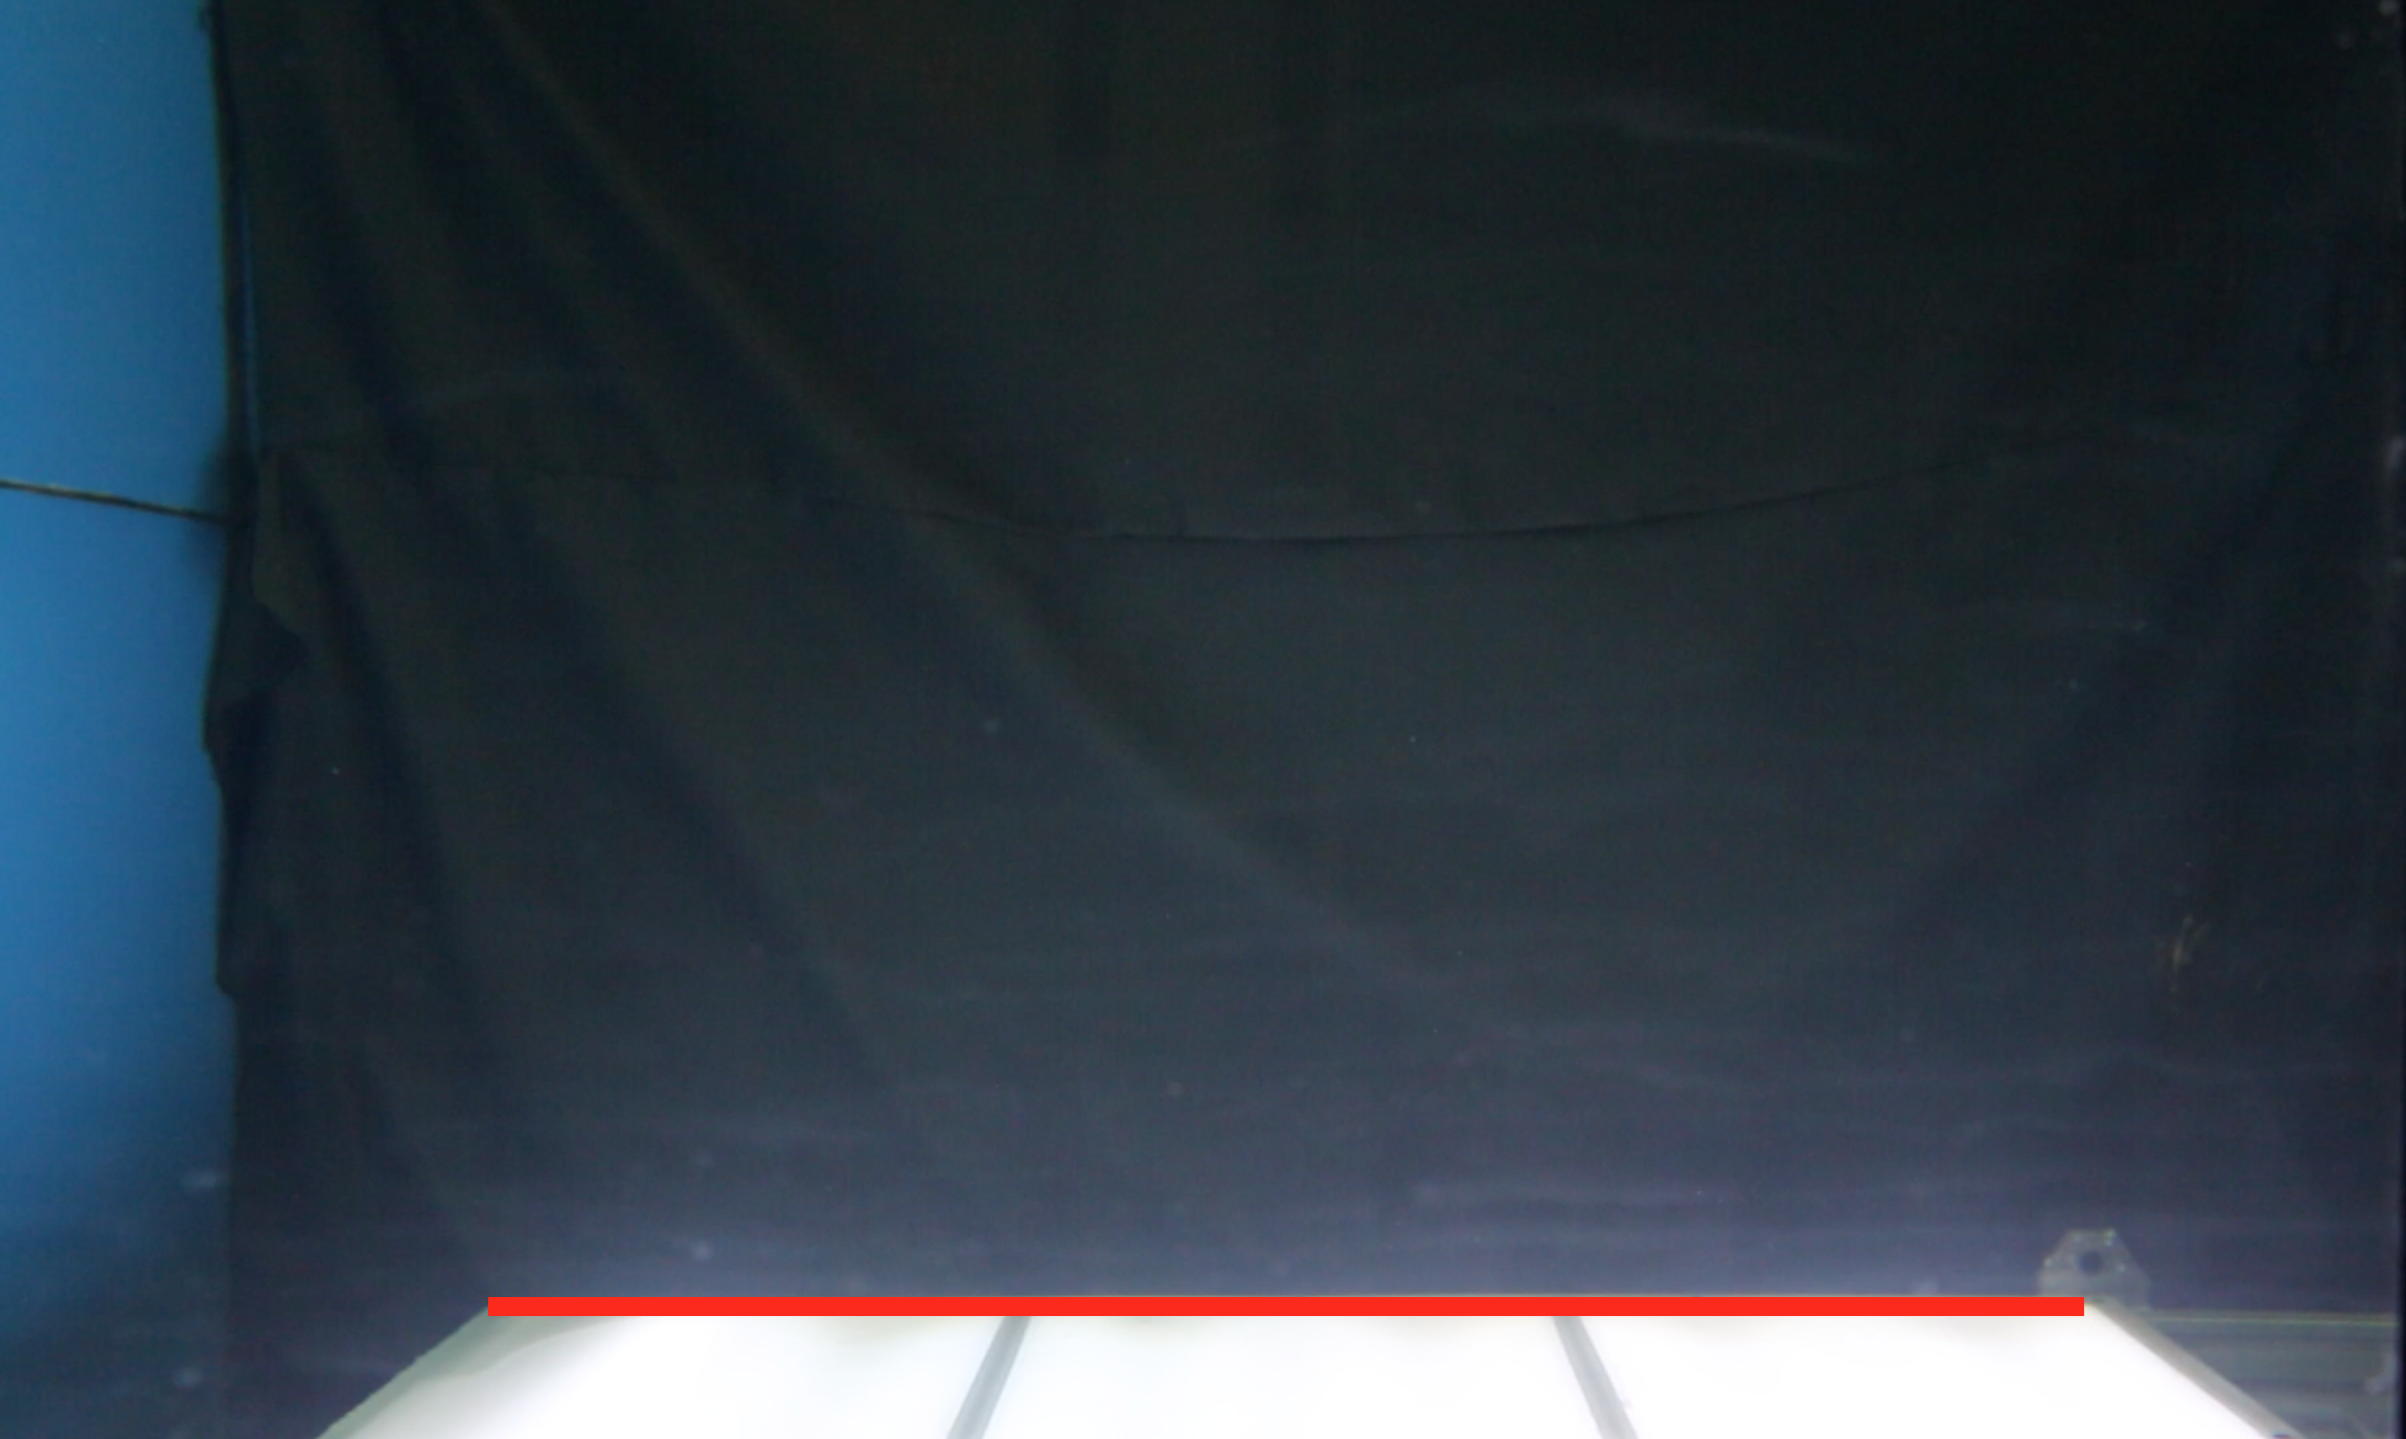
\includegraphics[width=0.8\textwidth]{Images/Traveltime_frame.png}
    \caption{Frame used to determine travel time}
    \label{fig:traveltime_frame}
\end{figure}





\begin{table}[ht!]
\centering
\begin{adjustbox}{max width = 0.8\linewidth}
\begin{tabular}{lllll|c|c|c|c|l|c|c|c|c|}
\cline{1-4} \cline{6-9} \cline{11-14}
\multicolumn{4}{|c|}{\textbf{Round}} &  & \multicolumn{4}{c|}{\textbf{Rectangular 20x3.9mm}} &  & \multicolumn{4}{c|}{\textbf{Rectangular 30x2.6mm}} \\ \cline{1-4} \cline{6-9} \cline{11-14} 
\multicolumn{1}{|l|}{\textbf{Test \#}} & \multicolumn{1}{l|}{\bm{$T_{start}$}} & \multicolumn{1}{l|}{\bm{$T_{plate}$}} & \multicolumn{1}{l|}{\textbf{$\Delta$}} &  & \multicolumn{1}{l|}{\textbf{Test \#}} & \multicolumn{1}{l|}{\bm{$T_{start}$}} & \multicolumn{1}{l|}{\bm{$T_{plate}$}} & \multicolumn{1}{l|}{\textbf{$\Delta$}} &  & \multicolumn{1}{l|}{\textbf{Test \#}} & \multicolumn{1}{l|}{\bm{$T_{start}$}} & \multicolumn{1}{l|}{\bm{$T_{plate}$}} & \multicolumn{1}{l|}{\textbf{$\Delta$}} \\ \cline{1-4} \cline{6-9} \cline{11-14} 
\multicolumn{1}{|c|}{1} & \multicolumn{1}{c|}{174} & \multicolumn{1}{c|}{208} & \multicolumn{1}{c|}{34} &  & 1 & 88 & 113 & 25 &  & 1 & 289 & 314 & 25 \\ \cline{1-4} \cline{6-9} \cline{11-14} 
\multicolumn{1}{|c|}{2} & \multicolumn{1}{c|}{182} & \multicolumn{1}{c|}{205} & \multicolumn{1}{c|}{23} &  & 2 & 70 & 101 & 31 &  & 2 & 60 & 90 & 30 \\ \cline{1-4} \cline{6-9} \cline{11-14} 
\multicolumn{1}{|c|}{3} & \multicolumn{1}{c|}{84} & \multicolumn{1}{c|}{110} & \multicolumn{1}{c|}{26} &  & 3 & 228 & 143 & 25 &  & 3 & 75 & 104 & 29 \\ \cline{1-4} \cline{6-9} \cline{11-14} 
\multicolumn{1}{|c|}{4} & \multicolumn{1}{c|}{90} & \multicolumn{1}{c|}{121} & \multicolumn{1}{c|}{31} &  & 4 & 440 & 466 & 26 &  & 4 & 75 & 98 & 23 \\ \cline{1-4} \cline{6-9} \cline{11-14} 
\multicolumn{1}{|c|}{5} & \multicolumn{1}{c|}{122} & \multicolumn{1}{c|}{154} & \multicolumn{1}{c|}{32} &  & 5 & 151 & 176 & 25 &  & 5 & 145 & 174 & 29 \\ \cline{1-4} \cline{6-9} \cline{11-14} 
 &  &  &  &  & 6 & 32 & 58 & 26 &  & 6 & 120 & 151 & 31 \\ \cline{6-9} \cline{11-14} 
 &  &  &  &  & 7 & 207 & 231 & 24 &  & 7 & 77 & 105 & 28 \\ \cline{6-9} \cline{11-14} 
 &  &  &  &  & 8 & 139 & 165 & 26 &  & 8 & 107 & 132 & 25 \\ \cline{6-9} \cline{11-14} 
 &  &  &  &  & 9 & 130 & 160 & 30 &  & 9 & 151 & 175 & 24 \\ \cline{6-9} \cline{11-14} 
 &  &  &  &  & 10 & 150 & 174 & 24 &  & 10 & 49 & 78 & 29 \\ \cline{6-9} \cline{11-14} 
 &  &  &  &  & 11 & 93 & 120 & 27 &  & 11 & 109 & 134 & 25 \\ \cline{6-9} \cline{11-14} 
 &  &  &  &  & 12 & 33 & 58 & 25 &  & 12 & 82 & 106 & 24 \\ \cline{6-9} \cline{11-14} 
 &  &  &  &  & 13 & 155 & 178 & 23 &  & 13 & 90 & 119 & 29 \\ \cline{6-9} \cline{11-14} 
 &  &  &  &  & 14 & 50 & 77 & 27 &  & 14 & 95 & 119 & 24 \\ \cline{6-9} \cline{11-14} 
 &  &  &  &  & 15 & 36 & 65 & 29 &  & 15 & 123 & 148 & 25 \\ \cline{6-9} \cline{11-14} 
 &  &  &  &  & 16 & 37 & 60 & 23 &  & 16 & 74 & 98 & 24 \\ \cline{6-9} \cline{11-14} 
 &  &  &  &  & 17 & 44 & 77 & 33 &  & 17 & 119 & 146 & 27 \\ \cline{6-9} \cline{11-14} 
 &  &  &  &  & 18 & 48 & 73 & 25 &  & 18 & 109 & 134 & 25 \\ \cline{6-9} \cline{11-14} 
 &  &  &  &  & 19 & 142 & 169 & 27 &  & 19 & 119 & 143 & 24 \\ \cline{6-9} \cline{11-14} 
 &  &  &  &  & 20 & 43 & 71 & 28 &  & 20 & 100 & 127 & 27 \\ \cline{6-9} \cline{11-14} 
\end{tabular}
\end{adjustbox}
\caption{Measured start times and time the plume reaches the back end of the plate for each nozzle shape}
\label{tab:traveltime}
\end{table}

\begin{table}[ht!]
\centering
\begin{adjustbox}{max width = 0.6\linewidth}
\begin{tabular}{|l|l|l|l|}
\hline
 & \textbf{Round} & \textbf{Rectangular 20x3.9mm} & \textbf{Rectangular 30x2.6mm} \\ \hline
\textbf{Average $\Delta$} & \multicolumn{1}{c|}{29.2} & \multicolumn{1}{c|}{26.45} & \multicolumn{1}{c|}{26.35} \\ \hline
\end{tabular}
\end{adjustbox}
\caption{Average measured $\Delta$ for the three nozzle shapes}
\label{tab:average_delta_traveltime}
\end{table}





\section{Summary}
%Concentration
%Aspect ratio
%Angles
%Entrainment coefficient


%Test uitslagen 
%Data verwerking
%Analytisch verantworoden